\documentclass[10pt, a4paper]{article}

\usepackage[utf8]{inputenc}
\usepackage[spanish]{babel} 
\usepackage[margin = 1in]{geometry} 
\usepackage{caratula}
\usepackage{algorithmicx}
\usepackage{algpseudocode}
\usepackage[Algoritmo]{algorithm}
\usepackage[fleqn]{amsmath}
\usepackage{color}
\usepackage{url}
\usepackage[colorlinks = true, linkcolor = blue]{hyperref}
\usepackage{comment}
\usepackage{hyperref}

\hypersetup{urlcolor=blue}

\makeatletter
\newenvironment{breakablealgorithm}
  {% \begin{breakablealgorithm}
   \begin{center}
     \refstepcounter{algorithm}% New algorithm
     \hrule height.8pt depth0pt \kern2pt% \@fs@pre for \@fs@ruled
     \renewcommand{\caption}[2][\relax]{% Make a new \caption
       {\raggedright\textbf{\ALG@name~\thealgorithm} ##2\par}%
       \ifx\relax##1\relax % #1 is \relax
         \addcontentsline{loa}{algorithm}{\protect\numberline{\thealgorithm}##2}%
       \else % #1 is not \relax
         \addcontentsline{loa}{algorithm}{\protect\numberline{\thealgorithm}##1}%
       \fi
       \kern2pt\hrule\kern2pt
     }
  }{% \end{breakablealgorithm}
     \kern2pt\hrule\relax% \@fs@post for \@fs@ruled
   \end{center}
  }
\makeatother


\begin{document}

\titulo{Trabajo práctico III}

\subtitulo{Camino mínimo a maestro Pokémon}

\materia{Algoritmos y Estructuras de Datos III}

\integrante{Bogdanich Espina, Vera}{601/14}{verabogdanichespina@gmail.com}
\integrante{Cámera, Joel Esteban}{257/14}{joel.e.camera@gmail.com}
\integrante{Gomez Gonzalez, Horacio Javier}{756/13}{horaciogomez.1993@gmail.com}
\integrante{Lavia, Alejandro Norberto}{43/11}{lavia.alejandro@gmail.com}

\maketitle

\tableofcontents

\newpage

\section{Ejercicio I: Algoritmo exacto}

\subsection{Introducci\'on}

Backtracking es una técnica para encontrar solución a algunos problemas computacionales, que incrementalmente construye candidatos a solución y abandona cada candidato parcial inmediatamente tras chequear que este no puede ser completado para generar una solución válida. Se utiliza en caso de que el problema admita como solución a un candidato ``parcial''.
Para esta solución pensamos a los gimnasios y paradas como nodos de un grafo completo donde los pesos de las aristas equivalen a la distancia entre los nodos.


\begin{comment}
A continuación se puede observar un psuedocódigo para la idea general de backtracking.
\begin{algorithm}[H]
\label{}
\caption{Idea general de backtracking}
\begin{algorithmic}[1]
\Statex \underline{Entrada}: S un conjunto de elementos que no forman parte de la soluci\'on parcial, N la lista de elementos de la soluci\'on parcial
\medskip
\If{solucionP(N)}
        \State nodosConsiderados $\gets$ nodos que forman el camino hallado por el algoritmo goloso
    }
    \Else
        \State nodosConsiderados $\gets$ nodos que representan a las pokeparadas del grafo
    \EndIf

\State s* $\gets$ s $\in$ S
\While{($\exists$ s $\in$ N(s*)) f(s) $<$ f(s*)}
    \State s* $\gets$ s $\in$ N(s*) tal que f(s) $<$ f(s*)
\EndWhile
\medskip
\Statex \underline{Salida}: s*
\end{algorithmic}
\end{algorithm}

procedure bt(c)
  if reject(P,c) then return
  if accept(P,c) then output(P,c)
  s ← first(P,c)
  while s ≠ Λ do
    bt(s)
    s ← next(P,s)

En el primer llamado a la función, S es el conjunto con todos los elementos que se podrían utilizar en una solución, y N es un conjunto vacío, ya que aún no se ha chequeado nada.
\end{comment}



\subsection{Algoritmo}

La solución que implementamos para obtener el camino óptimo es un backtracking. 
Para analizar cada camino utilizamos los siguientes criterios:
\begin{itemize}
    \item Si el camino que se está chequeando pasa por todos los gimnasios y recorre menos distancia que la mejor solucion encontrada hasta el momento, se reemplaza esa solución con el camino actual.
    \item Si la distancia del camino actual es mayor a la distancia del mejor encontrado, no se chequean mas caminos que partan de este.
    \item Si la distancia del camino actual es menor a la distancia del mejor hallado, y es un movimiento válido (en caso de ser un gimnasio el último nodo agregado al camino, habrá que chequear que las pociones fueran suficientes para vencerle); entonces se verifican todos los caminos que partan desde este último, sólo teniendo en cuenta como continuación los nodos que aún no están en el camino actual.
\end{itemize}

\begin{algorithm}[H]
\label{}
\caption{Backtracking}
\begin{algorithmic}[1]
\Statex \underline{Entrada}: distanciaActual: \texttt{float}, pociones: \texttt{int}, gimnasiosPorVisitar: \texttt{int}, recorridos: \texttt{cola}, restantes: \texttt{cola}, mejorSolucion{cola}
\medskip
\If{gimnasiosPorVisitar == 0}
    \If{distanciaActual < mejorSolucion.distancia}
        \State mejorSolucion $\gets$ recorridos
    \EndIf
\Else
    \If{distanciaActual < mejorSolucion.distancia}
        \State ultimo $\gets$ restantes.back
        \While{haya nodos para visitar}
            \State proximoAVisitar $\gets$ restantes.front
            \State restantes.pop
            \State dist $\gets$ distancia(recorridos.back, proximoAVisitar)
            \State recorridos.push(proximoAVisitar)

            \If{esGimnasio(proximoAVisitar)}
                \State backtracking(distanciaActual+dist,pociones-pociones(proximoAVisitar), gimnasiosPorVisitar-1, restantes, recorridos, mejorSolucion)
            \Else
                \State backtracking(distanciaActual+dist, min(pociones+3, mochila), gimnasiosPorvisitar, restantes, recorridos, mejorSolucion)
            \EndIf
        \EndWhile
    \EndIf
\EndIf
\medskip
\Statex \underline{Salida}: mejorSolucion.imprimirSoluci\'on
\end{algorithmic}
\end{algorithm}


\subsection{Complejidad}

El backtracking, a lo sumo chequea cada combinacion posible de gimnasios y paradas en todos sus ordenes posibles; lo que, dicho de otra manera serían todas las permutaciones de cada subconjunto de partes del conjunto de nodos. 
Como cada permutacion de longitud k se construye a partir de una permutación de longitud k-1, no necesitamos construir ningún camino más de una vez.
Esto nos lleva a ver que lo que recorremos es un arbol, donde la raíz es el "conjunto vacío" (no haber recorrido nada) y el camino simple desde la misma hasta cada hoja es una permutación diferente de longitud n, donde n es la cantidad de nodos.
Habiendo entendido esto, llegamos rapidamente a la conclusión de que nuestro backtracking pertenece a la clase de complejidad \bigo{n!} ya que construye a lo sumo todas las permutaciones de longitud n, las cuales contienen a todas las de tamaños menores.


\subsection{Experimentaci\'on}

Planteamos dos experimentos diferentes para el backtracking. Para ambos utilizamos instancias en las que los gimnasios representan un tercio de los nodos, y las paradas, los nodos restantes.

El primero consiste en corroborar que la cota teórica de complejidad calculada se cumple en la práctica. Para esto utilizamos instancias del problema en las que es necesario pasar por la totalidad de las paradas para poder vencer en todos los gimnasios (acomodando adecuadamente los requerimientos de pociones). 
A continuación observamos un gráfico en el que se refleja la división entre la función obtenida a partir de medir los ticks del clock en función de la cantidad de nodos y la función de complejidad

\begin{figure}[H]
  \begin{center}
    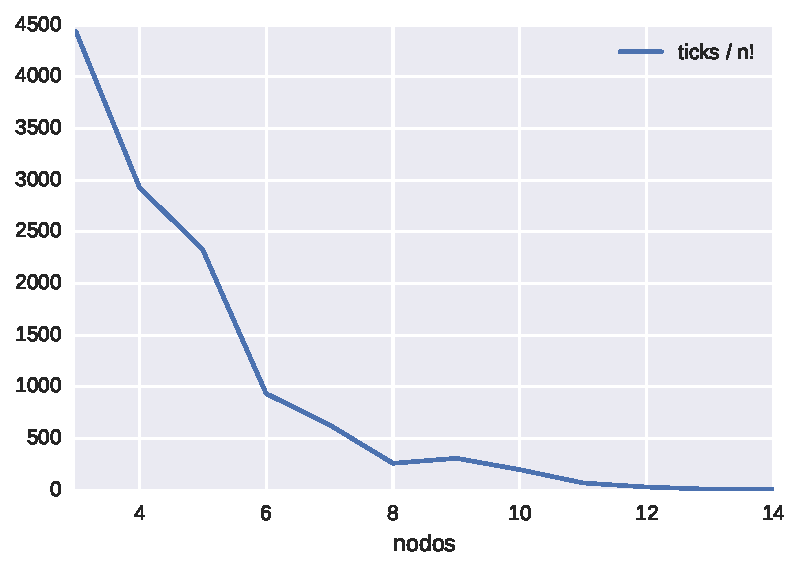
\includegraphics{../experimentacion/ej1/ej1_complejidad.pdf}
    \caption{Tiempo en ciclos sobre (cantidad de nodos)! en función de la cantidad de nodos.}
    \label{fig:ej1_complejidad}
  \end{center}
\end{figure}

Como podemos observar en la figura \ref{fig:ej1_complejidad}, la funcion N! / cantidad de ticks es decreciente, lo que muestra que N! acota superiormente a nuestra implementación.

Para el segundo experimento, definimos un parámetro de dificultad que representa el porcentaje de paradas necesarias para poder triunfar en todos los gimnasios. Creemos que a medida que aumenta esta dificultad, el backtracking tardará más en encontrar alguna solución viable y podará menos soluciones parciales, por lo que tomará más tiempo de ejecución.
Aquí debajo podemos ver un heatmap en el que mostramos la cantidad de ticks de reloj en función de la cantidad de nodos y de la dificultad.

\begin{figure}[H]
  \begin{center}
    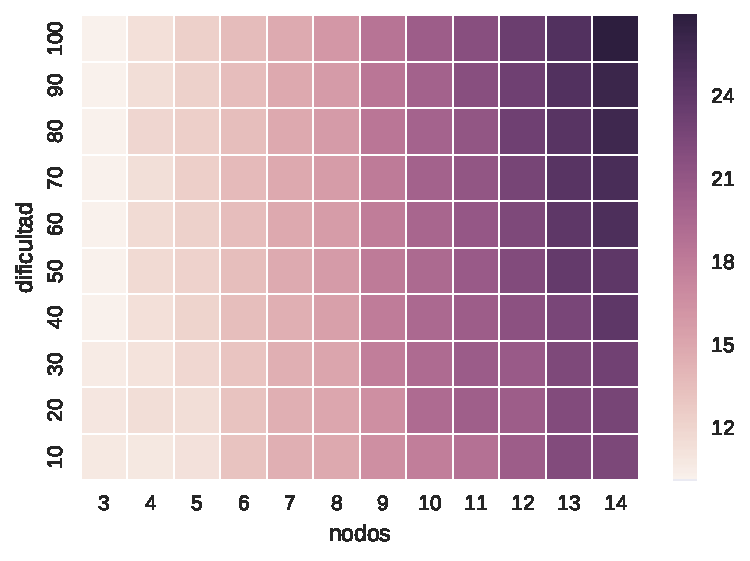
\includegraphics{../experimentacion/ej1/ej1_conHeuristica.pdf}
    \caption{Tiempo medido en ciclos en función de la cantidad de nodos y la dificultad.}
    \label{fig:ej1_conHeuristica}
  \end{center}
\end{figure}

Como podemos observar en la figura \ref{fig:ej1_conHeuristica}, la cantidad de ticks del clock aumenta en función de ambas variables, por lo que nuestra hipótesis está confirmada.

Para este último experimento, probamos utilizar la heurística del ejercicio 2 para hallar una distancia para usar como cota en el bactracking al realizar el primer llamado. Las mediciones realizadas tanto con la cota como sin la cota dieron muy similares, lo que nos llevo a entender que el backtracking hallaba una gran cantidad de soluciones con distancias menores que la encontrada por la heurística, por lo que el tiempo de cómputo no se vio afectado. 


\newpage

\section{Ejercicio II: Heurística constructiva golosa}

En el problema dado, Brian necesita conocer el camino con el menor recorrido para vencer a todos los gimnasios. Cómo sabe que buscar la solución óptima puede ser muy costosa se decide por generar una heurística para tener de forma más rápida una solución que, si bien no es la óptima, va a estar cercana a ella.

\subsection{Algoritmo}

La \textbf{heurística constructiva golosa} propuesta para obtener una solución es la de ir siempre al vecino más cercano. Cómo la mochila comienza vacía, siempre se comienza desde una poke parada. Entonces desde allí se pregunta si puede ganarle a algún gimnasio con las pociones que ya tiene, si puede ganarle se acerca hasta el gimnasio más cercano de los que puede ganar, guardándose la distancia y descartándose las pociones necesarias para derrotarlo; si no puede ganarle a ningún gimnasio se acerca hasta poke parada más cercana y agrega otras tres pociones a la mochila, si ésta lo permite, sino hasta llenarla. Luego, vuelve a preguntarse si puede ganarle a algún gimnasio y realiza los mismos pasos anteriores.

El algoritmo termina si no puede ganarle a ningún gimnasio y tiene la mochila llena, devolviendo $-1$; si no puede ganarle a ningún gimnasio y recorrió todas las poke paradas, también devolviendo $-1$; o si le ganó a todos los gimnasios, en ese caso devolviendo la distancia recorrida, la cantidad de gimnasios y poke paradas que recorrió y el camino recorrido.

Ahora bien, cómo comenzamos el algoritmo desde cualquier poke parada ésta podría generar una solución menos óptima que si comenzamos desde otra. Por ello, éste algoritmo se ejecuta una vez por cada poke parada comenzando siempre por alguna distinta y guardando la solución. Luego, se devuelve la mejor solución de las guardadas.

Por otra parte, analizamos una serie de casos particulares por separado al comienzo del algoritmo propuesto. Estos son casos donde ya se sabe de ante mano cual va a ser la solución y se puede llegar a ella con una complejidad menor, por ello las separamos y realizamos desde un comienzo. Los casos son los siguientes:

\begin{itemize}

\item Si no hay gimnasios: no hace falta recorrer nada. Se devuelve $0 0$.

\item Si $cantidadParadas*3 < sumaTotalDePocionesDeGimnasios$: No hay solución en este caso. Se devuelve $-1$.

\item Si no hay poke paradas o la mochila tiene capacidad $0$ y existe al menos un gimnasio donde su cantidad de pociones necesaria para ganarle es mayor que $0$: No hay solución. Se devuelve $-1$.

\item Si en todos los gimnasios la cantidad de pociones necesarias para ganarles es de $0$: Hay solución. En este caso corremos el mismo algorimo que detallamos antes pero, en vez de comenzar en poke paradas, comenzamos en gimnasios. Tomamos todas las soluciones y devolvemos la mejor.

\end{itemize}

Con todo esto descripto anteriormente, el pseudocódigo del algoritmo propuesto es el siguiente:

\begin{algorithm}[H]
\label{}
\caption{\textbf{SolucionHeuristicaGolosa}(\textbf{mochila}: entero, \textbf{gimnasios}: vector(gym), \textbf{paradas}: vector(parada))}
\begin{algorithmic}[1]

\If{esVacio(gimnasios)}
	\State Devolver $0$ $0$
	\State Terminar
\EndIf

\If{(cantidad(paradas)*3 $<$ SumaTodasLasPociones(gimnasios))}
	\State Devolver $-1$
	\State Terminar
\EndIf

\If{(esVacio(paradas) ó mochila $== 0$) y SumaTodasLasPociones(gimnasios) $> 0$}
	\State Devolver $-1$
	\State Terminar
\EndIf

\State Conj(solucion) c $\leftarrow$ Vacio()

\If{SumaTodasLasPociones(gimnasios) $== 0$}


	\For{cada g gimnasio en gimnasios}

		\State solucion s $\leftarrow$ SolucionCasoGeneral(g, mochila, paradas, gimnasios)

		\State Agregar(c,s)

	\EndFor

	\State DevolverMejorSolucion(c)
	\State Terminar
\Else

	\For{cada p parada en paradas}

		\State solucion s $\leftarrow$ SolucionCasoGeneral(p, mochila, paradas, gimnasios)

		\State Agregar(c,s)

	\EndFor

\EndIf

\State DevolverMejorSolucion(c)
\State Terminar

\medskip
\Statex \underline{}
\end{algorithmic}
\end{algorithm}
% \Statex \underline{Salida}:

Cómo se puede apreciar en el algoritmo, utilizamos un conjunto de soluciones pero no mencionamos nada de ellas. Para que se entienda mejor, para nosotros una solución es una tupla (entero, cola), donde el entero representa la distancia recorrida total y la cola es el camino recorrido.

También, gimnasio y parada son las tuplas mencionadas ya antes en la introducción pero a efectos de entender este pseudo código mejor repetiremos. Gimnasio es una tupla de la forma (x, y, pociones) y parada es una tupla de la forma de la forma (x, y). Los valores x e y son enteros que determinan la posición; pociones es un entero que referencia a la cantidad de pociones necesarias para ganarle al gimnasio; y visitado es un bool en

Ahora presentamos el pseudo código de la función SolucionCasoGeneral:

\begin{algorithm}[H]
\label{}
\caption{\textbf{SolucionCasoGeneral}(\textbf{nodoComienzo}: nodo, \textbf{mochila}: entero, \textbf{gimnasios}: vector(gym), \textbf{paradas}: vector(parada))}
\begin{algorithmic}[1]

\State solucion s $\leftarrow$ \{0, Vacia()\}

\If{nodoComienzo es un gimnasio}

	\State m $\leftarrow$ 0  // Valor de la mochila
	\State Marcar nodoComienzo como visitado en gimnasios

\Else

	\State m $\leftarrow$ 3  // Valor de la mochila
	\State Marcar nodoComienzo como visitado en paradas

\EndIf

\State Encolar(s.cola, nodoComienzo)

\For{Mientras no se hayan visitado todos los gimnasios}

	\If{Si le gano a algún gimnasio con las pociones que tengo}
		\State g $\leftarrow$ DameGimnasioMasCercanoQueGano(gimnasios)
		\State m $\leftarrow$ m - g.pociones
		\State ActualizarDistancia(s.distancia, g.distancia)
		\State Encolar(s.cola, g)
		\State Marcar a g como visitado en gimnasios

	\ElsIf{Si la mochila esta llena ó todas las paradas están recorridas}
		\State // Aquí no le gano a ningún gimnasio
		\State s.distancia $\leftarrow$ $-1$
		\State Retornar s
	
	\Else

		\State p $\leftarrow$ DameParadaMasCercana(paradas)
		\State ActualizarDistancia(s.distancia, p.distancia)
		\State Encolar(s.cola, p)
		\State Marcar a p como visitado en paradas

	\EndIf

\EndFor

\State retornar s

\medskip
\Statex \underline{}
\end{algorithmic}
\end{algorithm}
% \Statex \underline{Salida}:

Y con esto termina nuestro algoritmo propuesto con una \textbf{heurística constructiva golosa}.

Para no agobiar con tanto código, en esta sección no ahondaremos en el resto de las funciones auxiliares, que consideramos de por si declarativas, pero si haremos un análisis profundo de ellas en la siguiente sección donde analizaremos la complejidad del código.


\subsection{Calculo de complejidad}

En esta sección analizaremos en profundidad nuestra implementación del pseudo código presentado.

Antes de comenzar a hacer un análisis exhaustivo del mismo, y para que no generar repeticiones, hablaremos de las estructuras utilizadas en nuestra implementación.

\subsubsection{Estructuras utilizadas de la \textit{Standard Template Library} de C++}

En nuestra implementación utilizamos dos estructuras de la \textit{Standard Template Library} de C++: \emph{queue}\footnote{\url{http://www.cplusplus.com/reference/queue/queue/}} y \emph{vector}\footnote{\url{http://www.cplusplus.com/reference/vector/vector/}}.

De la estructura \emph{queue}, las funciones que utilizaremos son: push\footnote{\url{http://www.cplusplus.com/reference/queue/queue/push/}}, pop\footnote{\url{http://www.cplusplus.com/reference/queue/queue/pop/}}, front\footnote{\url{http://www.cplusplus.com/reference/queue/queue/front/}} y size\footnote{\url{http://www.cplusplus.com/reference/queue/queue/size/}}, donde la complejidad de las mismas es de tiempo constante.

De la estructura \emph{vector}, las funciones que utilizaremos son: el constructor que toma el tamaño como parametro de entrada\footnote{\url{http://www.cplusplus.com/reference/vector/vector/vector/}}, size\footnote{\url{http://www.cplusplus.com/reference/vector/vector/size/}} y el operador [] que devuelve el elemento i-ésimo\footnote{\url{http://www.cplusplus.com/reference/vector/vector/operator[]/}}. Las complejidades de size y el operador [] son constantes y la del constructor es lineal sobre el tamaño que se pasa como parametro.

% No me gusta este titulo
\subsubsection{Estructuras creadas por nosotros}

Hemos creado tres tipos de estructuras para ayudarnos en nuestra implementación, las cuales son: \textbf{gym} que tiene dos float que representan la posición, un entero que representa la cantidad de pociones necesarias para ganarle y un booleano para saber si el nodo fue visitado o no; \textbf{parada} que tiene dos float que representan la posición y un booleano para saber si fue visitado; y \textbf{solucion} que tiene un float que representa la distancia recorrida hasta el momento y una cola donde guardamos el camino recorrido de dicha distancia


% No me gusta como están dispuestos los titulos, modificar
\subsubsection{Analisis de complejidad}


Ahora si pasamos a hacer un examen exhaustivo para el cálculo de la complejidad de nuestra implementación. Para realizarlo comenzaremos primero con la función \textbf{SolucionCasoGeneral} para luego obtener mejor la complejidad de la función \textbf{SolucionHeuristicaGolosa}.

Cabe aclarar desde un comienzo que, como el grafo modelado es completo, generamos desde un comienzo una matriz de adyacencia con el peso de la arista en cada nodo (o sea, la distancia entre dos nodos). De ésta matriz hablaremos, junto con su complejidad, cuando analicemos la función \textbf{SolucionHeuristicaGolosa} pero mencionamos ahora porque utilizamos ésta matriz para obtener la distancia entre dos nodos en $\mathcal{O}(1)$.


\subsubsection{Función SolucionCasoGeneral}

Analizaremos con detalle cada parte de esta función. Para esto, iremos tomando porciones del pseudo código enunciado antes y explicando como funcionan en nuestra implementación, así obtener la complejidad. Algo que cabe destacar es la aridad de ésta función en nuestra implementación. La misma es: 

~
\textbf{SolucionCasoGeneral}(\textbf{nodoComienzo}: nodo, \textbf{s} solucion, \textbf{mochila}: entero, \textbf{gimnasios}: vector(gym), \textbf{paradas}: vector(parada)) $\rightarrow$ \textit{void}
~

Donde la solución es la estructura comentada anteriormente que pasamos por referencia. Ésta viene con distancia cero y la cola vacía.

Comencemos el análisis de la complejidad:

\begin{algorithm}[H]
\label{}
\begin{algorithmic}[]

\State solucion s $\leftarrow$ \{0, Vacia()\}

\If{nodoComienzo es un gimnasio}

	\State m $\leftarrow$ 0  // Valor de la mochila
	\State Marcar nodoComienzo como visitado en gimnasios

\Else

	\State m $\leftarrow$ 3  // Valor de la mochila
	\State Marcar nodoComienzo como visitado en paradas

\EndIf

\State Encolar(s.cola, nodoComienzo)

\medskip
\Statex \underline{}
\end{algorithmic}
\end{algorithm}


Lo que primero que realiza el pseudo código es generar la estructura solución vacía, pero como ésta se recibe como parametro no realizamos la operación en nuestra implementación.

Luego, observamos si el nodoComienzo es un gimnasio o una parada. nodoComienzo es el índice de entrada del nodo (la entrada toma primero 1..n nodos gimnasios y, luego, (n+1)..m nodos paradas). Si es menor que n es un gimnasio y si es mayor es una parada. Saber esto es $\mathcal{O}(1)$.

Cómo cada nodoComienzo es un índice, podemos marcar al mismo cómo visitado poniendo \textit{true} en su vector, con una complejidad constante, y luego le asignamos un número al m que representa la mochila. Esto lo hace tanto en la rama del \textit{if} como en la del \textit{else}, por lo tanto la complejidad de ambas ramas es la misma.

Por último, se encola el elemento en la cola de la solución que, como vimos anteriormente tiene complejidad constante.

Entonces, mostramos un pseudo código más cercano a nuestra implementación con la complejidad de la parte analizada:

\begin{algorithm}[H]
\label{}
\begin{algorithmic}[]

\State solucion s $\leftarrow$ \{0, Vacia()\} \Comment{$\mathcal{O}(1)$}

\If{nodoComienzo es un gimnasio} \Comment{$\mathcal{O}(1)$}

	\State m $\leftarrow$ 0  \Comment{$\mathcal{O}(1)$}
	\State gimnasios[nodoComienzo].visitado $\leftarrow$ true \Comment{$\mathcal{O}(1)$}
\Else

	\State m $\leftarrow$ 3  \Comment{$\mathcal{O}(1)$}
	\State paradas[nodoComienzo].visitado $\leftarrow$ true \Comment{$\mathcal{O}(1)$}

\EndIf

\State Encolar(s.cola, nodoComienzo) \Comment{$\mathcal{O}(1)$}

\medskip
\Statex \underline{Complejidad: $\mathcal{O}(1) + \mathcal{O}(1) + \mathcal{O}(1) + \mathcal{O}(1) + \mathcal{O}(1) = \mathcal{O}(1)$}
\end{algorithmic}
\end{algorithm}


Seguimos con la siguiente parte del código:

\begin{algorithm}[H]
\label{}
\begin{algorithmic}[]

\For{Mientras no se hayan visitado todos los gimnasios}

	\If{Si le gano a algún gimnasio con las pociones que tengo}
		\State g $\leftarrow$ DameGimnasioMasCercanoQueGano(gimnasios)
		\State m $\leftarrow$ m - g.pociones
		\State ActualizarDistancia(s.distancia, g.distancia)
		\State Encolar(s.cola, g)
		\State Marcar a g como visitado en gimnasios

	\ElsIf{Si la mochila esta llena ó todas las paradas estan recorridas}
		\State // Si entro aquí no hay solución
		\State s.distancia $\leftarrow$ $-1$
		\State Retornar s
	
	\Else

		\State p $\leftarrow$ DameParadaMasCercana(paradas)
		\State ActualizarDistancia(s.distancia, p.distancia)
		\State Encolar(s.cola, p)
		\State Marcar a p como visitado en paradas

	\EndIf

\EndFor

\State retornar s

\medskip
\Statex \underline{}
\end{algorithmic}
\end{algorithm}


En ésta porción del código hay partes que no son triviales, por ende iremos analizandolas una por una con sumo detalle.

En la guarda del For dice \textit{Mientras no se hayan visitado todos los gimnasios}. Para esto tenemos un entero llamado \emph{gym\_no\_recorridos} que se inicializa desde un comienzo con la cantidad de gimnasios y cada vez que se visita alguno se actualiza restandole uno. Por lo tanto, saber si se visitaron todos los gimnasios tiene como complejidad $\mathcal{O}(1)$.

Analicemos cada condición del if:

La primera guarda dice \textit{Si le gano a algún gimnasio con las pociones que tengo}. Para esta guarda generamos una función que se llama \textbf{leGanoAAlgunGym}, que toma por referencia al vector gimnasios, en donde recorre linealmente al vector mirando si alguno no fue visitado y en tal caso, si le puedo ganar con la cantidad de pociones que tengo. Si encuentra alguno devuelve true, sino false.
Un pseudo código de la función sería de esta forma:
\[
	\text{\textbf{Función} leGanoAAlgunGym:}
\]
\[
	\text{\textbf{return: }} \exists (i \leftarrow |gimnasios|) \neg gimnasios[i].visitado \land gimnasios[i].p \leq mochila
\]

Como recorre de forma lineal el vector de gimnasios, su complejidad es $\mathcal{O}(|gimnasios|)$.

Si ésta devuelve verdadero, entra en el bloque donde  se busca el gimnasio más al que se le puede ganar y se actualizan todas las variables relacionadas. Para esta parte generamos una función llamada \textbf{leGanoAlGymMasCercano}, que toma por referencia a la solución, el vector de gimnasios y la matriz de distancias; y donde realiza todas estas operaciones en conjunto de la siguiente forma:

\begin{itemize}
	\item Recorro de forma lineal los gimnasios buscando un gimnasio que no haya sido visitado, al que le pueda ganar y sea el más cercano. Esto se hace obteniendo un gimnasio que es el mejor en el momento y, si encontramos otro que cumpla con esto y sea más cercano, lo cambiamos por el que teníamos, y continuamos con esta operatoria hasta recorrerlos a todos. Saber si fue visitado o si le puedo ganar tiene como complejidad $\mathcal{O}(1)$ y la distancia entre dos nodos también es $\mathcal{O}(1)$. Por lo tanto, su complejidad es $\mathcal{O}(|gimnasios|)$.
	\item Una vez que obtengo el gimnasio, actualizo la mochila $\mathcal{O}(1)$.
	\item Actualizo la distancia de la solución $\mathcal{O}(1)$.
	\item Meto en la cola de la solución el nodo del gimnasio $\mathcal{O}(1)$.
	\item Marcamos como visitado al gimnasio en el vector, asignándole true al flag de visitado. $\mathcal{O}(1)$
	\item Restamos uno a la variable \emph{gym\_no\_recorridos}.
\end{itemize}

Por lo tanto, la complejidad de este bloque de código es: $\mathcal{O}(|gimnasios|) + \mathcal{O}(1) + \mathcal{O}(1) + \mathcal{O}(1) + \mathcal{O}(1) = \mathcal{O}(|gimnasios|)$.

La segunda guarda del if dice \textit{Si la mochila esta llena ó todas las paradas están recorridas}. Esta guarda tiene complejidad $\mathcal{O}(1)$ ya que el valor de la mochila es un entero y puedo saber si llegó al máximo valor con una simple comparación. Para saber si las paradas fueron visitadas, cómo hicimos con los gimnasios, tenemos un entero llamado \emph{paradas\_no\_recorridas}, donde al comienzo de la función se le asigna la cantidad de paradas y cada vez que se pasa por alguna se le resta uno. Entonces, para saber si recorrí todas las paradas es una saber si \emph{paradas\_no\_recorridas} es igual que cero y la complejidad es $\mathcal{O}(1)$. Por lo tanto, la complejidad de la guarda es $\mathcal{O}(1)$.

Si esta segunda guarda tiene como resultado verdadero, entra a un bloque donde se le asigna a la distancia de la solución el valor de $-1$ y termina la ejecución del programa. Por lo tanto, este bloque tiene como complejidad $\mathcal{O}(1)$.

Por último, si las guardas anteriores dan falso, entra al bloque del else. Dentro lo que hace es obtener la parada más cercana, actualizar la distancia, encolar la parada y marcarla como visitada. Para realizar esto creamos una función llamada \textbf{voyParadaMasCercana}, que toma una referencia a la estructura solución, una referencia al vector de paradas, el valor límite de la mochila y una referencia a la matriz de distancias. La forma de realizar estas operaciones es la siguiente:

\begin{itemize}

	\item Para obtener la parada más cercana realizamos una operación similar a la de la función \textbf{leGanoAlGymMasCercano}. Recorremos en forma lineal al vector de paradas buscado una parada que no haya sido visitada y que su distancia sea la más cercana. Cuando obtenemos una, seguimos buscando hasta el final para ver si se puede mejorar y cambiarla por la mejor. Por lo tanto, su complejidad es $\mathcal{O}(|paradas|)$
	\item Una vez obtenida la parada mas cercana, actualizamos la mochila sumándole tres, o lo necesario para llegar hasta el tope. $\mathcal{O}(1)$
	\item Sumamos la distancia a la solución. $\mathcal{O}(1)$
	\item Marcamos la parada como visitada en el vector. $\mathcal{O}(1)$
	\item Restamos en uno a la variable \emph{paradas\_no\_recorridas}. $\mathcal{O}(1)$

\end{itemize}

Sumando todas las complejidades de esta función queda la siguiente complejidad: $\mathcal{O}(|paradas|) + \mathcal{O}(1) + \mathcal{O}(1) + \mathcal{O}(1) + \mathcal{O}(1) = \mathcal{O}(|paradas|)$.

Por lo tanto, la parte de código analizada con sus complejidades quedaría de la siguiente forma:

\begin{algorithm}[H]
\label{}
\begin{algorithmic}[]

\While{gym\_no\_recorridos $> 0$} \Comment{$\mathcal{O}(1)$}

	\If{leGanoAAlgunGym(gimnasios)} \Comment{$\mathcal{O}(|gimnasios|)$}

		\State leGanoAlGymMasCercano(s, gimnasios, matriz) \Comment{$\mathcal{O}(|gimnasios|)$}

	\ElsIf{m == mochila $\land$ paradas\_no\_recorridas == 0} \Comment{$\mathcal{O}(1)$}
		\State s.distancia $\leftarrow$ $-1$ \Comment{$\mathcal{O}(1)$}
		\State Retornar \Comment{$\mathcal{O}(1)$}
	
	\Else

		\State voyParadaMasCercana(mochila, s, paradas, matriz) \Comment{$\mathcal{O}(|Paradas|)$}

	\EndIf

\EndWhile

\State Retornar \Comment{$\mathcal{O}(1)$}

\medskip
\Statex \underline{}
\end{algorithmic}
\end{algorithm}


Para cada gimnasio hay que tener las pociones suficientes en la mochila para ganarle, entonces se necesita al menos pasar por una poke parada antes de ir a un gimnasio. Por lo tanto, ese ciclo se realiza la cantidad de gimnasios más la cantidad de poke paradas, o sea, la cantidad total de nodos del grafo. Esto daría como complejidad total: $\mathcal{O}(N)* ( 2*\mathcal{O}(|gimnasios|) + \mathcal{O}(1) + \mathcal{O}(|paradas|) = \mathcal{O}(N) * (max\{\mathcal{O}(|gimnasios|), \mathcal{O}(|paradas|)\})$. Siendo $N$ la cantidad total de nodos del grafo (gimnasios + paradas).

Para finalizar el análisis de ésta función, unamos la complejidad de las dos partes para obtener la complejidad total de la misma: Por la primera parte tenemos $\mathcal{O}(1)$ y por la última $\mathcal{O}(N) * (max\{\mathcal{O}(|gimnasios|), \mathcal{O}(|paradas|)\})$. Por lo tanto, la complejidad total de la función está dada por la última parte.

Complejidad de la función \textbf{SolucionCasoGeneral} es de: $\mathcal{O}(N) * (max\{\mathcal{O}(|gimnasios|), \mathcal{O}(|paradas|)\})$.


\subsubsection{Función SolucionHeuristicaGolosa}


En ésta función haremos el análisis de la misma forma que la anterior, iremos tomando porciones de código y analisandolas en detalle y por separado obteniendo la complejidad de cada una de ellas, para luego unir las complejidades y obtener así la complejidad total de la función.

Antes de comenzar, cabe aclarar que difiere un poco la descripción de la función que haremos a la implementación real, pero no así en complejidad. Con esto nos referimos a que agregaremos una funcionalidad más hacia el final de la misma que es imprimir la solución. En nuestra implementación lo que hacemos es devolver la estructura solución e imprimirla por fuera, esto es para poder utilizarla en los siguientes ejercicios de este trabajo y como es la única operación que hacemos por fuera nos parece razonable incluirla dentro y hacer este comentario.

Comencemos el análisis.

Lo primero que realiza nuestra implementación, y que no está en el pseudo código, es generar una matriz de adyacencias donde en sus coordenadas tenemos la distancia entre los nodos. Generamos ésta matriz para optimizar un poco este cálculo. Un pseudo código de la creación de la misma es:

\[
	\text{\textbf{return}:  } M \text{ donde } M \in \mathbb{R}^{NxN} \text{ y } (\forall i \in \text{filas($M$)})(\forall j \in \text{columnas($M$)}) M[i,j] = distancia(nodo[i], nodo[j])
\]

Siendo $N$ la cantidad total de nodos del grafo y nodo[] representa a cada nodo del mismo, pudiendo ser tanto un gimnasio como una parada. Generar ésta matriz tiene un costo de $\mathcal{O}(N^2)$.

Esto es lo único distinto en el comienzo de nuestro pseudo código con la implementación original. Continuemos con el análisis de la primera parte del algoritmo:

\begin{algorithm}[H]
\label{}
\begin{algorithmic}[]

\If{esVacio(gimnasios)}
	\State Devolver $0$ $0$
	\State Terminar
\EndIf

\If{(cantidad(paradas)*3 $<$ SumaTodasLasPociones(gimnasios))}
	\State Devolver $-1$
	\State Terminar
\EndIf

\If{(esVacio(paradas) ó mochila $== 0$) y SumaTodasLasPociones(gimnasios) $> 0$}
	\State Devolver $-1$
	\State Terminar
\EndIf

\medskip
\Statex \underline{}
\end{algorithmic}
\end{algorithm}

Para toda esta primera parte del pseudo código generamos una función que se llama \textbf{SolucionCasosParticulares} donde encapsula todas estas operaciones más el siguiente if de la función que lo analizamos con la siguiente parte. Ésta tiene como parametros la máxima cantidad de pociones que puede llevar la mochila, el vector gimnasios, el vector paradas, la matriz de adyacencias y una solución.

Lo primero que realiza es ver si la cantidad de gimnasios es $0$, esto se realiza con la función size del tipo vector que tiene como complejidad $\mathcal{O}(1)$. Si esto es verdadero, lo que hace es devolver $0 0$ y salir, en la implementación le asignamos a la distancia un $0$ y terminamos la ejecución. Complejidad de este if con su bloque es $\mathcal{O}(1)$.

Luego, observamos si la cantidad de paradas por tres es menor estricto que la suma de las pociones necesarias de los gimnasios para ganarles. Si ocurre esto, el caso no tiene solución. Saber cual es la cantidad de paradas lo hacemos utilizando la función size en $\mathcal{O}(1)$. Saber cual es la suma de las pociones necesarias para ganarle a los gimnasios ya no es trivial, debemos recorrerlos a todos. Por ello lo calculamos antes en nuestra implementación. Un pseudo código del calculo sería:

\[
	\text{\textbf{return: }} \sum_{i \in |gimnasios|} gimnasios[i].p
\]
Éste calculo tiene complejidad $\mathcal{O}(|gimnasios|)$.

Entonces si ésta guarda es verdadera, realiza una operación parecida a la del if anterior con la diferencia de que, como este caso no tiene solución, asignamos a la distancia un $-1$ y terminamos la ejecución. Complejidad de éste segundo if con el bloque es $\mathcal{O}(|gimnasios|) + \mathcal{O}(1) = \mathcal{O}(|gimnasios|)$.

El siguiente if es parecido al recién visto en términos de complejidad, si no hay paradas o la mochila tiene una capacidad nula para las pociones y hay algún gimnasio en el que se requiere como mínimo una poción para ganarle entonces no hay solución y el bloque del if es el mismo que el anterior. Saber si no hay paradas con la función size tiene complejidad $\mathcal{O}(1)$, saber si la mochila tiene capacidad nula también es $\mathcal{O}(1)$ y la suma de las pociones necesarias de los gimnasios para ganarles ya fue calculada, por lo tanto la complejidad del if con el bloque es de $\mathcal{O}(1)$.

Por lo tanto, un pseudo código  más cerca de la realidad junto con la complejidad sería:

\begin{algorithm}[H]
\label{}
\begin{algorithmic}[]

\If{esVacio(gimnasios)} \Comment{$\mathcal{O}(1)$}
	\State sol.d $\leftarrow 0$ \Comment{$\mathcal{O}(1)$}
	\State Terminar \Comment{$\mathcal{O}(1)$}
\EndIf

\State suma $\leftarrow$ SumaTodasLasPociones(gimnasios) \Comment{$\mathcal{O}(|gimnasios|)$}

\If{cantidad(paradas)*3 $<$ suma} \Comment{$\mathcal{O}(1)$}
	\State sol.d $\leftarrow -1$ \Comment{$\mathcal{O}(1)$}
	\State Terminar
\EndIf

\If{(esVacio(paradas) ó mochila $== 0$) y suma $> 0$} \Comment{$\mathcal{O}(1)$}
	\State Devolver $-1$ \Comment{$\mathcal{O}(1)$}
	\State Terminar
\EndIf

\medskip
\Statex \underline{Complejidad: $\mathcal{O}(1) + \mathcal{O}(|gimnasios|) + \mathcal{O}(1) + \mathcal{O}(1) = \mathcal{O}(|gimnasios|)$}
\end{algorithmic}
\end{algorithm}

Ahora analisemos la segunda y última parte del código:

\begin{algorithm}[H]
\label{}
\begin{algorithmic}[]

\State Conj(solucion) c $\leftarrow$ Vacio()

\If{SumaTodasLasPociones(gimnasios) $== 0$}

	\For{cada g gimnasio en gimnasios}

		\State solucion s $\leftarrow$ SolucionCasoGeneral(g, mochila, paradas, gimnasios)

		\State Agregar(c,s)

	\EndFor

\Else

	\For{cada p parada en paradas}

		\State solucion s $\leftarrow$ SolucionCasoGeneral(p, mochila, paradas, gimnasios)

		\State Agregar(c,s)

	\EndFor

\EndIf

\State DevolverMejorSolucion(c)
\State Terminar

\medskip
\Statex \underline{}
\end{algorithmic}
\end{algorithm}

Como podemos observar, se realiza casi el mismo código tanto si la guarda del if es verdadera como falsa, así que iremos analisandolo al mismo tiempo.

Lo primero es la complejidad de la guarda del if, como la suma de las pociones de todos los gimnasios la tenemos calculada de un principio, ésta es $\mathcal{O}(1)$.

Luego, cada for itera sobre la cantidad de gimnasios en el primer bloque o paradas en el segundo y, como cada una de estas es un índice, la complejidad de la guarda en cada una de las iteraciones es $\mathcal{O}(1)$.

Dentro de cada for se hace un llamado a la función \textbf{SolucionCasoGeneral}, por cada gimnasio o parada dependiendo en que bloque corra, y donde la complejidad ya fue calculada: $\mathcal{O}(N) * (max\{\mathcal{O}(|gimnasios|), \mathcal{O}(|paradas|)\})$ siendo $N$ la cantidad de nodos, y se la misma en el conjunto de solución creado.

En nuestra implementación no tenemos un conjunto de soluciones sino que tenemos un puntero a solución que comparamos con la que devuelve la función \textbf{SolucionCasoGeneral}, si es mejor que la que tenemos la cambiamos, sino seguimos buscando hasta el final, la comparación se hace con respecto a la distancia recorrida, por lo tanto ésta es $\mathcal{O}(1)$ y, como es un puntero, simplemente intercambiar punteros también es $\mathcal{O}(1)$.

Analicemos que cambios tiene la complejidad si la guarda del if es verdadera o falsa, ya que el código es similar. Si la guarda es verdadera, quiere decir que no se necesita ninguna poción para ganarle a ningún gimnasio, por ende, corremos la función \textbf{SolucionCasoGeneral} desde todos los gimnasios buscando la mínima distancia. Por como esta hecha la función, siempre va a encontrar un gimnasio al que ganarle y avanzaría hasta el más cercano, nunca pasaría por las poke paradas. Esto hace que la complejidad de la función no sea $\mathcal{O}(N) * (max\{\mathcal{O}(|gimnasios|), \mathcal{O}(|paradas|)\})$, sino $\mathcal{O}(|gimnasios|) * \mathcal{O}(|gimnasios|) = \mathcal{O}(|gimnasios|^2)$. Y, cómo esta función se realiza por cada gimnasio, la complejidad de éste bloque es: $\mathcal{O}(|gimnasios|)* \mathcal{O}(|gimnasios|^2) = \mathcal{O}(|gimnasios|^3)$.

Si la guarda es falsa, entonces necesitaría, como mínimo, pasar por una poke parada para poder ir a algún gimnasio. Por lo tanto, la complejidad de la función \textbf{SolucionCasoGeneral} es la calculada previamente $\mathcal{O}(N) * (max\{\mathcal{O}(|gimnasios|), \mathcal{O}(|paradas|)\})$. Y, cómo esta función se realiza por cada parada, la complejidad de éste bloque es: $\mathcal{O}(|paradas|) \mathcal{O}(N) * (max\{\mathcal{O}(|gimnasios|), \mathcal{O}(|paradas|)\})$.

Por último, despues de obtener la mejor solución, y cómo dijimos en un principio que lo hacíamos por fuera pero lo agregamos aquí a sólo hecho del cálculo de la complejidad, es imprimir esa solución. Para imprimir generamos la función \textbf{imprimirSolucion} donde imprimimos la distancia y luego vamos desencolando e imprimiendo el índice de cada nodo. Cómo en peor caso se recorren todos los nodos, la complejidad de ésta función es $\mathcal{O}(N)$, siendo $N$ la cantidad de nodos.

Un pseudo código más cercano a la realidad y con las complejidades seria de la siguiente forma:

\begin{algorithm}[H]
\label{}
\begin{algorithmic}[]

\State solucion* mejor\_sol \Comment{$\mathcal{O}(1)$}

\If{SumaTodasLasPociones(gimnasios) $== 0$} \Comment{$\mathcal{O}(1)$}

	\For{cada g gimnasio en gimnasios} \Comment{$\mathcal{O}(1)$}

		\State solucion s $\leftarrow$ SolucionCasoGeneral(g, mochila, paradas, gimnasios) \Comment{$\mathcal{O}(|gimnasios|^2)$}

		\If{s.d < mejor\_sol.d} \Comment{$\mathcal{O}(1)$}
			\State mejor\_sol = s \Comment{$\mathcal{O}(1)$}
		\EndIf
	
	\EndFor
	\Comment{Complejidad total del for $\mathcal{O}(|gimnasios|^3)$}

\Else

	\For{cada p parada en paradas} \Comment{$\mathcal{O}(1)$}

		\State solucion s $\leftarrow$ SolucionCasoGeneral(p, mochila, paradas, gimnasios) \Comment{$\mathcal{O}(|gimnasios|) * \mathcal{O}(N)$}

		\If{s.d < mejor\_sol.d} \Comment{$\mathcal{O}(1)$}
			\State mejor\_sol = s \Comment{$\mathcal{O}(1)$}
		\EndIf

	\EndFor
	\Comment{Complejidad total del for $\mathcal{O}(|paradas|) * \mathcal{O}(|gimnasios|) * \mathcal{O}(N)$}


\EndIf

\State imprimirSolucion(mejor\_sol) \Comment{$\mathcal{O}(N)$}
\State Terminar

\medskip
\Statex \underline{Complejidad: $\mathcal{O}(|gimnasios|^3) + \mathcal{O}(|paradas|) * \mathcal{O}(N) * (max\{\mathcal{O}(|gimnasios|), \mathcal{O}(|paradas|)\}) + \mathcal{O}(N)$}
\end{algorithmic}
\end{algorithm}

Por lo tanto, la complejidad de la función, y total de la solución propuesta, es la suma total de las complejidades $\mathcal{O}(N^2) + \mathcal{O}(|gimnasios|^3) + \mathcal{O}(|paradas|) * \mathcal{O}(N) * (max\{\mathcal{O}(|gimnasios|), \mathcal{O}(|paradas|)\}) + \mathcal{O}(N) = max\{\mathcal{O}(N^2), \mathcal{O}(|gimnasios|^3), \mathcal{O}(|paradas|) * \mathcal{O}(N) * (max\{\mathcal{O}(|gimnasios|), \mathcal{O}(|paradas|)\})\}$.






\newpage

\section{Ejercicio III: Heur\'istica de b\'usqueda local}

\subsection{Introducci\'on}
\label{sec:ej3_intro}

B\'usqueda local es un m\'etodo que parte de una soluci\'on no \'optima a un problema e intenta mejorarla a trav\'es de modificaciones, es decir, convirti\'endola en una soluci\'on \textit{vecina}. Luego, es necesario determinar qu\'e constituye una soluci\'on vecina a otra dada, hay que definir un \textit{vecindario}. Por ejemplo, en nuestro problema a resolver, donde una soluci\'on s* es un camino simple, que cumple ciertas condiciones, entre algunos nodos de un grafo, una soluci\'on vecina s a s* podr\'ia ser un camino id\'entico al de s* excepto por un nodo n que se reemplaza con otro n' que s* no recorre. Donde el reemplazo se interpreta como avanzar en s desde el predecesor de n en s* hacia n' y luego continuar por el siguiente de n en s*.

Presentamos a continuaci\'on un pseudoc\'odigo que ilustra la idea general de este algoritmo, en \'el asumimos que queremos minimizar f(s) donde s es una soluci\'on y f una funci\'on que la eval\'ua.

\begin{algorithm}[H]
\label{}
\caption{Idea general de b\'usqueda local}
\begin{algorithmic}[1]
\Statex \underline{Entrada}: S un conjunto de soluciones, N una funci\'on que devuelve las soluciones vecinas a otra dada y f una funci\'on que eval\'ua una soluci\'on
\medskip
\State s* $\gets$ s $\in$ S
\While{($\exists$ s $\in$ N(s*)) f(s) $<$ f(s*)}
    \State s* $\gets$ s $\in$ N(s*) tal que f(s) $<$ f(s*)
\EndWhile
\medskip
\Statex \underline{Salida}: s*
\end{algorithmic}
\end{algorithm}

\subsection{Algoritmo}

Para implementar una heur\'istica de b\'usqueda local para nuestro problema utilizamos una clase llamada \texttt{Camino} que est\'a formada por un grafo (en nuestra implementaci\'on son instancias de la clase \texttt{Grafo}), el tamaño de la mochila, la distancia computada hasta el momento y un puntero al primer nodo del grafo visitado en el recorrido actual, siendo todos los nodos elementos del tipo \texttt{Nodo}.

La clase \texttt{Grafo} est\'a compuesta por un vector de nodos y una matriz con la distancia entre cada par de nodos. Esta distancia se corresponde con la distancia euclideana\footnote{\url{https://es.wikipedia.org/wiki/Distancia_euclidiana}} calculada utilizando sus coordenadas.

Cada instancia de \texttt{Nodo} tiene un n\'umero de identificaci\'on, sus coordendas x e y, la cantidad de pociones que demanda u otorga, un valor booleano que indica si el nodo representa a un gimnasio, un puntero a su nodo anterior y otro a su nodo siguiente dentro del camino actual.

Luego, utilizando las estructuras descriptas anteriormente, realizamos una implementaci\'on que \textit{soporta} dos criterios distintos de vecindad:

\paragraph{Vecindad I: Permutaci\'on del camino}
Establecemos que s* es una soluci\'on vecina a s si el camino de s* se puede obtener permutando el orden en el que se recorren dos nodos en s. Este criterio se conoce comunmente como \textit{swap}.

\paragraph{Vecindad II: Permutaci\'on y reemplazo de las pokeparadas}
Este vecindario considera que s* es una soluci\'on vecina a otra s si el camino de s* es igual al de s luego de permutar el orden en el que se recorren dos pokeparadas, o reemplazar una pokeparada del camino por otra que no se encontraba en \'el. La motivaci\'on principal de esta vecindad fue suponer que una heur\'istica golosa podr\'ia encontrar un buen camino entre los gimnasios pero tendr\'ia dificultades estableciendo los \textit{desv\'ios} para buscar pociones.

\paragraph{}
Como explicamos en la secci\'on \ref{sec:ej3_intro}, para realizar una b\'usqueda local tomamos una soluci\'on incial que luego es \textit{mejorada}. Para esto decidimos utilizar el algoritmo goloso desarrollado en el segundo ejercicio.

Adem\'as, optamos por considerar tambi\'en las soluciones que devuelven una misma distancia final cuando no podemos encontrar soluciones vecinas que reduzcan ese n\'umero. Esperamos que en algunos casos esto nos permita hallar mejoras nuevas. Para evitar entrar en ciclos infinitos, por ejemplo, donde vamos de una soluci\'on s* a otra s equivalente, y de ella nuevamente volvemos a s*, utilizamos un diccionario donde tenemos como clave la identificaci\'on de un nodo y como significado un conjunto con las identificaciones de los nodos que fueron permutados o reemplazados por el primero. De esta manera tambi\'en limitamos la cantidad de soluciones equivalentes para analizar.

Todo lo descripto anteriormente se encuentra resumido en el siguiente pseudoc\'odigo:

\begin{algorithm}[H]
\label{}
\caption{B\'usqueda local}
\begin{algorithmic}[1]
\Statex \underline{Entrada}: camino : \texttt{Camino} y criterio : \texttt{Vecindad}
\medskip
\State camino.asignarSoluci\'onGolosa()
\If{camino.encontr\'eCamino()}
    \If{criterio == permutaCamino}
        \State nodosConsiderados $\gets$ nodos que forman el camino hallado por el algoritmo goloso
    \Else
        \State nodosConsiderados $\gets$ nodos que representan a las pokeparadas del grafo
    \EndIf
    \State busco $\gets$ true
    \State dicc(int, conj(int)) nodosCambiados $\gets$ Vac\'io()
    \While{busco}
        \While{camino.encuentroSoluci\'onVecinaMejor(nodosConsiderados)}
            \If{\#nodosCambiados.claves() $>$ 0}
                \State nodosCambiados $\gets$ Vac\'io()
            \EndIf
        \EndWhile
        \If{$\neg$camino.encuentroSoluci\'onVecinaIgual(nodosConsiderados, nodosCambiados)}
            \State busco $\gets$ false
        \EndIf
    \EndWhile
\EndIf
\medskip
\Statex \underline{Salida}: camino.imprimirSoluci\'on()
\end{algorithmic}
\end{algorithm}

Como podemos observar en las l\'ineas 12 y 13, si encuentro una soluci\'on que mejora la que ten\'ia vac\'io el diccionario por si ven\'ia de modificar mi camino por otro de distancia igual. Los ciclos \'unicamente ocurren cuando recorro soluciones equivalentes entre si.

Es importante destacar que la funci\'on \texttt{encuentroSoluci\'onVecinaMejor} devuelve el valor booleano \texttt{true} si encuentra una, y realiza las modificaciones necesarias en la instancia de \texttt{Camino} para transformar la soluci\'on actual en la vecina hallada. Como el comportamiento de \texttt{encuentroSoluci\'onVecinaIgual} es an\'alogo, sumando la consulta al diccionario que recibe como argumento para evitar ciclos, exihibimos \'unicamente un psuedoc\'odigo de \texttt{encuentroSoluci\'onVecinaMejor}:

\begin{algorithm}[H]
\label{}
\caption{Encuentro una soluci\'on vecina mejor}
\begin{algorithmic}[1]
\Statex \underline{Entrada}: nodosConsiderados : \texttt{vector(Nodo)}
\medskip
\State busco $\gets$ true
\For{i = 0, ..., nodosConsiderados.tamaño()}
    \For{j = 0, ..., nodosConsiderados.tamaño()}
        \If{i $\neq$ j $\land$ (est\'aEnElCamino(nodosConsiderados[i]) $\lor$ est\'aEnElCamino(nodosConsiderados[j])) $\land$ cambiarMejora(nodosConsiderados[i], nodosConsiderados[j]))}
            \State busco $\gets$ false
        \EndIf
    \EndFor
\EndFor
\medskip
\Statex \underline{Salida}: $\neg$busco
\end{algorithmic}
\end{algorithm}

En s\'intesis, el algoritmo anterior toma cada par de nodos perteneciente al vector recibido y, apenas encuentra un par con un elemento que est\'a en el camino actual y que permite mejorar la distancia actual con su reemplazo o permutaci\'on, realiza la modificaci\'on, si esta fuera posible, y devuelve \texttt{true}. Que uno de los nodos no est\'e en el camino actual significa que mis nodos considerados son pokeparadas y estoy contemplando hacer un reemplazo, sino es una permutaci\'on del camino. \texttt{cambiarMejora} eval\'ua la distancia nueva luego de la modificaci\'on, si es menor a la actual y el cambio es posible, lo realiza y retorna \texttt{true}.

\begin{figure}[H]
  \begin{center}
    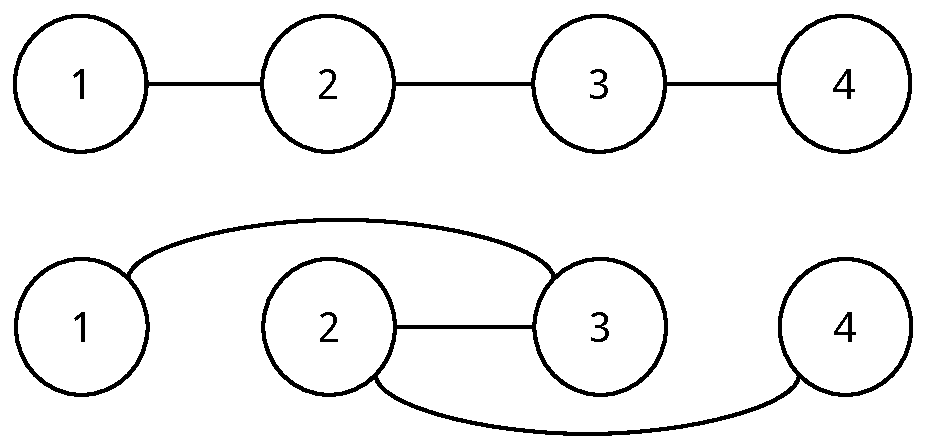
\includegraphics[scale = 0.5]{imagenes/ej3_algoritmo_1.pdf}
    \caption{Permutaci\'on de los nodos 2 y 3 en un camino posible del grafo.}
    \label{fig:ej3_algoritmo_1}
  \end{center}
\end{figure}

Para calcular la distancia nueva utilizamos los punteros almacenados en cada nodo. Si, por ejemplo, estuvi\'eramos en el caso de la figura \ref{fig:ej3_algoritmo_1} el c\'alculo realizado ser\'ia:
\begin{equation*}
distancia\ nueva = distancia\ actual - distancia(1,2) - distancia(3,4) + distancia(1,3) + distancia(2,4)
\end{equation*}

\begin{figure}[H]
  \begin{center}
    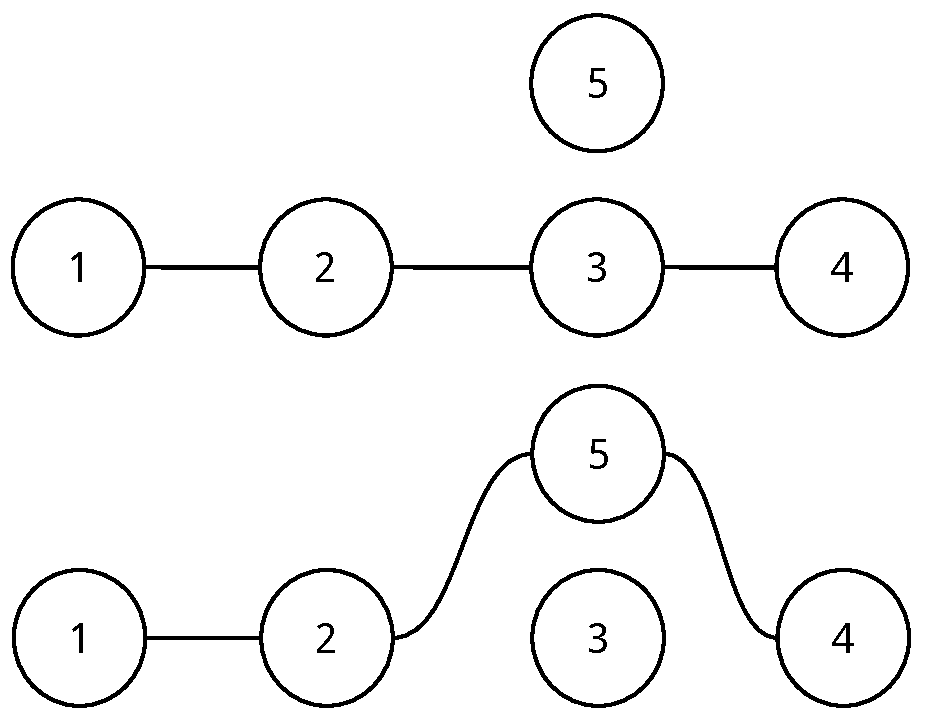
\includegraphics[scale = 0.5]{imagenes/ej3_algoritmo_2.pdf}
    \caption{Reemplazo del nodo 3 por el 5 en un camino posible del grafo.}
    \label{fig:ej3_algoritmo_2}
  \end{center}
\end{figure}

Si la modificaci\'on fuera un reemplazo, como, por ejemplo, en la figura \ref{fig:ej3_algoritmo_2}:
\begin{equation*}
distancia\ nueva = distancia\ actual - distancia(2,3) - distancia(3,4) + distancia(2,5) + distancia(5,4)
\end{equation*}

Analizamos si el reemplazo o la permutaci\'on es posible teniendo en cuenta las pociones que requieren los gimnasios, las que otorgan las pokeparadas y la capacidad de nuestra mochila. Con este fin avanzamos desde el nodo inicial de nuestra instancia de \texttt{Camino}, llevando la cuenta de cu\'antas pociones tenemos en nuestra mochila. Si el nodo actual es una pokeparada sumamos el m\'inimo entre 3 y lo que le reste de espacio a la mochila, en caso contrario restamos el costo del gimnasio. Si nuestra mochila queda con pociones negativas significa que el cambio no es posible y paramos de iterar, si no continuamos hasta llegar al final del camino. Llegar al nodo que no tiene siguiente significa que el cambio es posible.

\subsection{Complejidad}

El orden de complejidad temporal de peor caso para una iteraci\'on de la b\'usqueda local que mejora una soluci\'on, es decir, para encontrar una soluci\'on vecina s a s* tal que f(s) $<$ f(s*), es \bigo{k^2 \times $tamaño del camino$}, siendo k el tamaño de \texttt{nodosConsiderados}. En la primer vecindad esta complejidad es equivalente a \bigo{($tamaño del camino$)^3} $\in$ \bigo{(n+m)^3} siendo n la cantidad de gimnasios y m la cantidad de pokeparadas. Mientras que la complejidad de la vecindad que permuta y reemplaza pokeparadas es \bigo{m^2 \times $tamaño del camino$} $\in$ \bigo{m^2 \times (n+m)}.

Este tipo de iteraci\'on se corresponde con una ejecuci\'on de \texttt{encuentroSoluci\'onVecinaMejor}, all\'i para cada par de los elementos que componen \texttt{nodosConsiderados} evaluamos si realizar la modificaci\'on nos permite hallar una soluci\'on vecina mejor. En el peor caso no encontramos una hasta la \'ultima iteraci\'on del primer ciclo, es decir, realizamos $k^2$ iteraciones. En cada una de las iteraciones realizamos una llamada a \texttt{cambiarMejora} donde se calcula la distancia nueva con una cantidad constante de operaciones \bigo{1}. Si es menor a la distancia actual analiza si el cambio es posible con un costo de \bigo{$tamaño del camino$} $\in$ \bigo{n+m} en el pero caso, cuando el cambio es posible y recorre el camino completo sin obtener una cantidad \textit{negativa} de pociones. Por otra parte, el costo de \texttt{est\'aEnElCamino} es \bigo{1} porque simplemente revisa que los atributos \texttt{anterior} y \texttt{siguiente} del nodo no sean ambos inv\'alidos. El costo de realizar efectivamente el reemplazo o la permutaci\'on es \bigo{1} porque tambi\'en \'unicamente altera los atributos \texttt{anterior} y \texttt{siguiente} de los nodos a modificar, y los de sus dos vecinos.

Por otro lado, el orden de complejdidad de peor caso para una iteraci\'on de la b\'usqueda local que encuentra una soluci\'on vecina equivalente es \bigo{(n+m)^3 \times log(n+m)} en la vecindad que \'unicamente permuta y \bigo{m^2 \times (n+m) \times log(n+m)} en la restante.

En este caso una iteraci\'on de la b\'usqueda local se corresponde con una ejecuci\'on de \texttt{encuentro\\ Soluci\'onVecinaIgual}. Como explicamos anteriormente, es equivalente al algoritmo ya descripto, la \'unica diferencia recide en la guarda del \texttt{if}, para evitar ciclos en este caso tambi\'en revisa que nodosConsiderados[j].id $\notin$ nodosCambiados.significado(nodosConsiderados[i].id). En la implementaci\'on utilizamos el m\'etodo \texttt{count} de la clase \texttt{map} y el de la clase \texttt{set}, contenidas en la Standard Template Library de C++, para comprobar si nodosConsiderados[i] est\'a definido en nodosCambiados y luego si nodosConsiderados[j] est\'a contenido en su significado. Ambas operaciones tienen un costo logar\'itmico en funci\'on del tamaño del contenedor\footnote{\url{http://www.cplusplus.com/reference/map/map/count/} y \url{http://www.cplusplus.com/reference/set/set/count/}}. El diccionario tiene como m\'aximo k claves y sus significados en el peor caso son conjuntos de cardinal k.

Ejecutar nuestro algoritmo de b\'usqueda local sobre una soluci\'on inicial produce una cantidad de iteraciones de ambos tipos que no podemos estimar te\'oricamente. En pr\'oxima secci\'on intentamos encontrar una relaci\'on entre el n\'umero de iteraciones y los par\'ametros que recibe nuestro programa.

\subsection{Experimentación}

% GENERAL: Realizar una experimentacion computacional para medir la performance del programa implementado. Para ello se debe preparar un conjunto de casos de test que permitan observar los tiempos de ejecucion en funcion de los parametros de entrada. Deber ́an desarrollarse tanto experimentos con instancias aleatorias (detallando como fueron generadas) como experimentos con instancias particulares (de peor/mejor caso en tiempo de ejecuci ́on, por ejemplo). Se debe presentar adecuadamente en forma grafica una comparaci on entre los tiempos medidos y la complejidad te ́orica calculada y extraer conclusiones de la experimentaci ́on.
% una experimentacion b ́asica que muestre que la cota planteada de complejidad tiene sentido.
% algun experimento que muestre que el mejor caso es bueno y el peor caso es malo.
% otros experimentos que les parezcan relevantes y pongan de manifiesto alguna caracter ́ıstica del algoritmo (que ya deber ́ıan haber comentado en algun lado).
% una explicacion y justificacion de como van a hacer el experimento (como van a generar las instancias de prueba, cu ́antas corridas de cada uno van a tomar, etc.)

% ESTE TP: Realizar una experimentacion que permita observar la performance del algoritmo comparando
% los tiempos de ejecucion y la calidad de las soluciones obtenidas, en funci ́on de las vecindadeS utilizadas y elegir, si es posible, la configuraci ́on que mejores resultados provea para el grupo de instancias utilizado.Si es posible, dar una cota superior para la cantidad de iteraciones de la heur ́ıstica.

\subsubsection{Instancias estudiadas}

Con el objetivo de estudiar los algoritmos propuestos realizamos mediciones con diversos tipos de instancias que permiten hallar una soluci\'on por medio de la heur\'istica golosa que estudiamos anteriormente.

En cada medici\'on registramos: la cantidad de gimnasios, la cantidad de pokeparadas, el tamaño de la mochila, la distancia obtenida con la soluci\'on golosa, la distancia mejorada con una b\'usqueda local, la cantidad de permutaciones realizadas para mejorar la soluci\'on actual, la cantidad de permutaciones para cambiar la soluci\'on actual por otra igualmente buena, la cantidad de reemplazos para mejorar la soluci\'on actual, la cantidad de reemplazos para cambiar la soluci\'on actual por otra igualmente buena, el tamaño final del camino y el tiempo demorado en ciclos de reloj.

Para cada tipo creamos una cantidad fija de instancias de \texttt{Camino} y ejecutamos el algoritmo 100 veces. Cuando intentamos comparar nuestras soluciones con el \'optimo obtenido con backtracking ejecutamos este algoritmo 10 veces.

\paragraph{Instancias aleatorias}
Para generar cada instancia elegimos un n\'umero aleatorio de gimnasios entre 1 y 100. A cada gimnasio se le fij\'o una cantidad de pociones entre 0 y 10. Luego, sumamos las pociones que fueron asignadas a todos los gimnasios y elegimos una cantidad de pokeparadas random entre (cantidad total de pociones / 3) + 1 y ((cantidad total de pociones / 3) + 1) $\times$ 2. Las coordenadas de las pokeparadas y de los gimnasios se eligieron como n\'umeros aleatorios entre 0 y 1000. El tamaño de la mochila se determin\'o en 12 para evitar el desperdicio de pociones, debido a que lo m\'aximo que puede requerir un gimnasio es 10 pociones. Para estudiar este tipo creamos 30 instancias.

\paragraph{Instancias aleatorias y sus soluciones \'optimas}
Creamos 18 instancias con 1, 2, ..., 17 y 18 nodos cada una. En cada una elegimos la cantidad de gimnasios como el m\'inimo entre un n\'umero aleatorio entre 1 y la cantidad de nodos, y 10. Los nodos restantes corresponden a pokeparadas. Luego, establecemos que la cantidad m\'axima de pociones que puede pedir un gimnasio es (cantidad de pokeparadas $\times$ 3) / cantidad de gimnasios, y a cada nodo de tipo gimnasio le asignamos una cantidad de pociones aleatoria entre 1 y el m\'inimo entre 10 y el m\'aximo calculado para la instancia. Nuevamente, las coordenadas se eligieron aleatoriamente entre 0 y 1000, y el tamaño de la mochila se fij\'o en 12. Elegimos estas cantidades de 
gimnasios y pokeparadas para poder ejecutar el algoritmo de backtracking sobre estas instancias en un tiempo razonable.

\paragraph{Instancias de mejor caso}
Esperamos que la heur\'istica golosa tenga grandes dificultades para hallar caminos cercanos al \'optimo cuando los gimnasios y las pokeparadas se encuentran en \'areas distintas, ya que en primer lugar busca un camino entre los gimnasios y luego recorre las pokeparadas, lo que causar\'ia una ida y vuelta constante entre ambas \'areas. Estos casos, que podr\'iamos considerar como los \textit{peores} de la heur\'istica golosa, se corresonden con unos de los \textit{mejores} de la b\'usqueda local. Es decir, la b\'usqueda local va a tener un porcentaje de mejora mucho mayor que en instancias aleatorias. Para generarlas procedemos de forma an\'aloga que con las aleatorias, la \'unica diferencia es que los gimnasios ahora tienen como coordenadas n\'umeros entre 0 y 500, y las pokeparadas entre 500 y 1000. Adem\'as, el tamaño de la mochila se elige como la cantidad total de pociones que requieren los gimnasios, lo que permite recorrer primero el \'area de pokeparadas y luego el \'area de gimnasios. Nuevamente, generamos 30 instancias de este tipo.

\paragraph{Instancias de mejor caso y sus soluciones \'optimas}
Con el objetivo de generar este tipo de instancias procedemos de forma an\'aloga a los \'ultimos dos tipos descriptos. Separamos los gimnasios de las pokeparadas y generamos grafos de pocos nodos para poder ejecutar el algoritmo de backtracking.

\paragraph{Instancias con \#gimnasios fija e instancias con \#pokeparadas fija}
En este caso a la variable fija se le asigna el n\'umero 10 y para la restante se elije aleatoriamente otro entre 1 y 100, el tamaño de la mochila es 12 otra vez y creamos 30 instancias. Para determinar la cantidad de pociones que requieren los gimnasios hacemos lo mismo que cuando queremos estudiar soluciones \'optimas y generamos los caminos con un n\'umero fijo de gimnasios y pokeparadas.

\subsubsection{Complejidades}

Para comprobar emp\'iricamente las complejidades te\'oricas dividimos el tiempo de ejecuci\'on por la complejidad respectiva esperando encontrar una funci\'on constante. Estos datos se pueden apreciar con mayor claridad utilizando un \textit{boxplot} con su respectiva densidad:

\begin{figure}[H]
  \begin{center}
    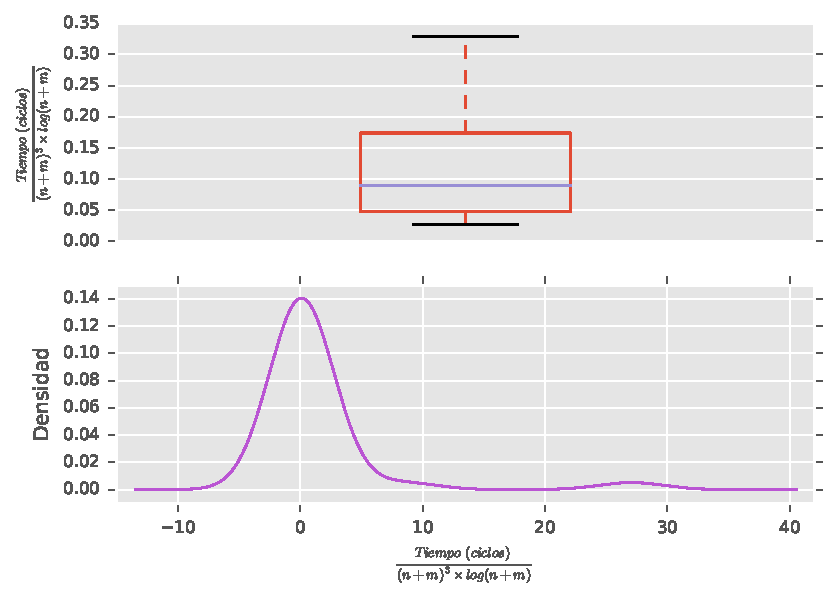
\includegraphics{../experimentacion/ej3/expAleat_complejidad_permutaCamino.pdf}
    \caption{Tiempo / complejidad en funci\'on de la cantidad de nodos para la vecindad que permuta el camino, utilizando instancias aleatorias.}
    \label{fig:expAleat_complejidad_permutaCamino}
  \end{center}
\end{figure}

\begin{figure}[H]
  \begin{center}
    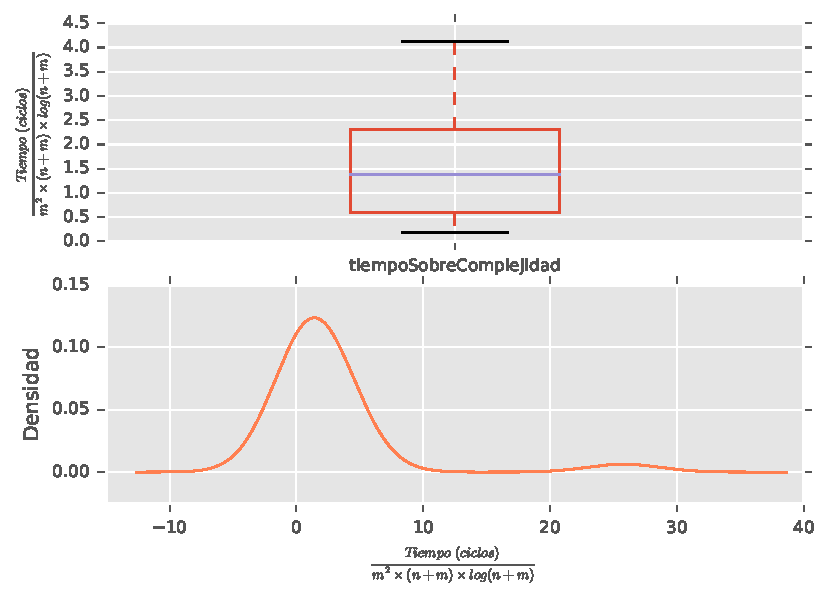
\includegraphics{../experimentacion/ej3/expFijo_complejidad_permutaYReemplazaPokeparadas_cantGimFija.pdf}
    \caption{Tiempo / complejidad en funci\'on de la cantidad de nodos para la vecindad que permuta y reemplaza pokeparadas, utilizando una cantidad de gimnasios fija.}
    \label{fig:expFijo_complejidad_permutaYReemplazaPokeparadas_cantGimFija}
  \end{center}
\end{figure}

\begin{figure}[H]
  \begin{center}
    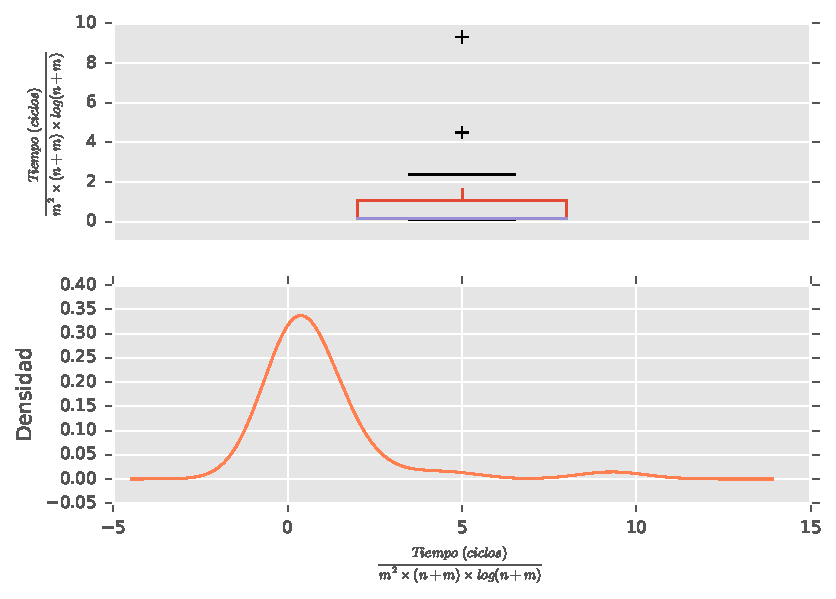
\includegraphics{../experimentacion/ej3/expFijo_complejidad_permutaYReemplazaPokeparadas_cantPokFija.pdf}
    \caption{Tiempo / complejidad en funci\'on de la cantidad de nodos para la vecindad que permuta y reemplaza pokeparadas, utilizando una cantidad de pokeparadas fija.}
    \label{fig:expFijo_complejidad_permutaYReemplazaPokeparadas_cantPokFija}
  \end{center}
\end{figure}

Como podemos observar en las figuras \ref{fig:expAleat_complejidad_permutaCamino}, \ref{fig:expFijo_complejidad_permutaYReemplazaPokeparadas_cantGimFija} y \ref{fig:expFijo_complejidad_permutaYReemplazaPokeparadas_cantPokFija} ...

\subsubsection{\#iteraciones de la b\'usqueda}

\begin{figure}[H]
  \begin{center}
    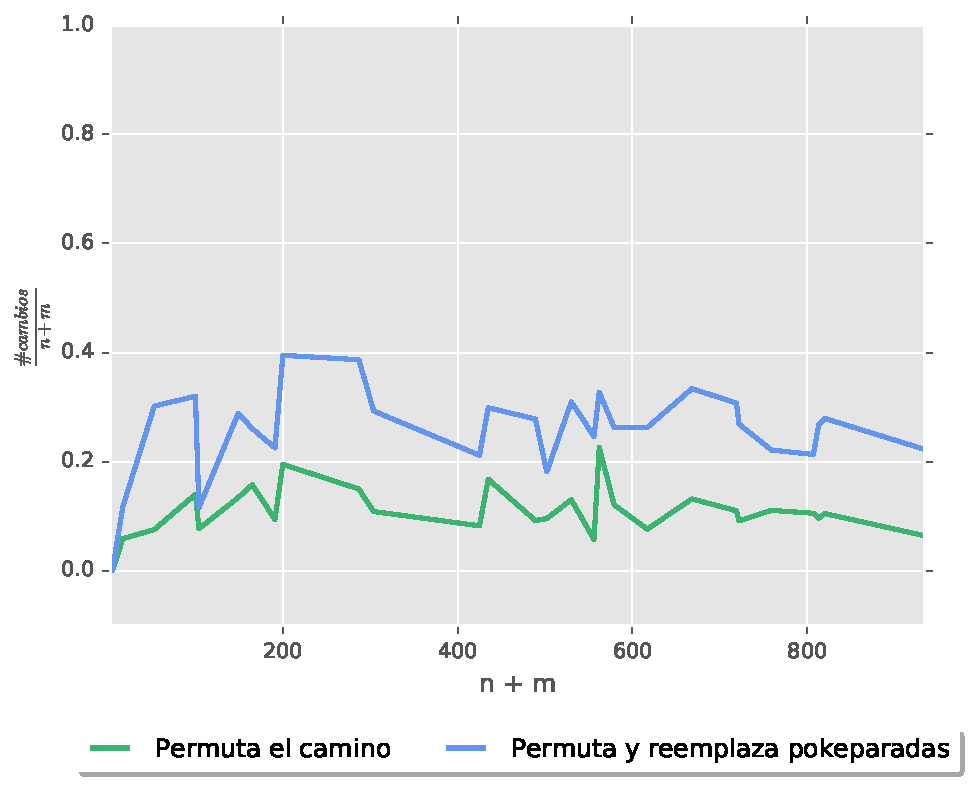
\includegraphics{../experimentacion/ej3/expAleat_cantCambios.pdf}
    \caption{expAleat cantCambios}
    \label{fig:expAleat_cantCambios}
  \end{center}
\end{figure}

\begin{figure}[H]
  \begin{center}
    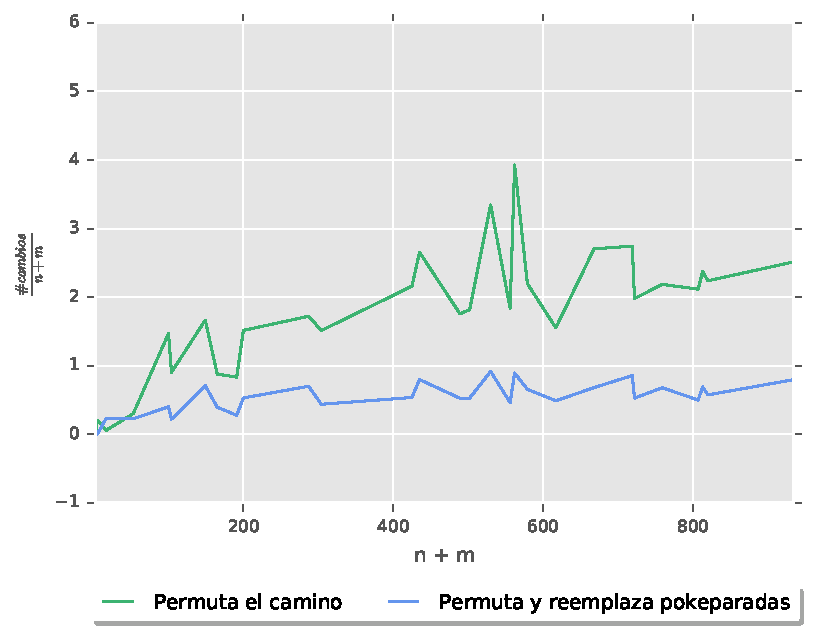
\includegraphics{../experimentacion/ej3/expMejor_cantCambios.pdf}
    \caption{expMejor cantCambios}
    \label{fig:expMejor_cantCambios}
  \end{center}
\end{figure}

\subsubsection{Calidad de las soluciones}

\begin{table}[H]
    \begin{center}
        \begin{tabular}{ | l | l | l | l | l | }
            \hline
            \multicolumn{1}{|c|}{}&
            \multicolumn{2}{|c|}{\textbf{Instancias aleatorias}}&
            \multicolumn{2}{|c|}{\textbf{Instancias de mejor caso}}\\
            \cline{2-5}
                            &    \textit{Vecindad I}     &    \textit{Vecindad II}    &    \textit{Vecindad I}     &    \textit{Vecindad II}    \\ \hline
            Media           &    11.368223  &   21.943365   &   70.201509   &    8.155963   \\ \hline
            Desv\'io estandar       &   3.848846    &    6.707769   &   20.632809   &   3.791787    \\ \hline
            M\'inimo        &   0.000000    &    0.000000   &   0.000000    &   0.000000    \\ \hline
            M\'aximo        &   18.463784   &    28.902765  &       84.686633   &    23.047859  \\ \hline
        \end{tabular}
    \end{center}
    \caption{Porcentaje de mejora.}    
    \label{table:porcentaje_mejora}
\end{table} 

\begin{figure}[H]
  \begin{center}
    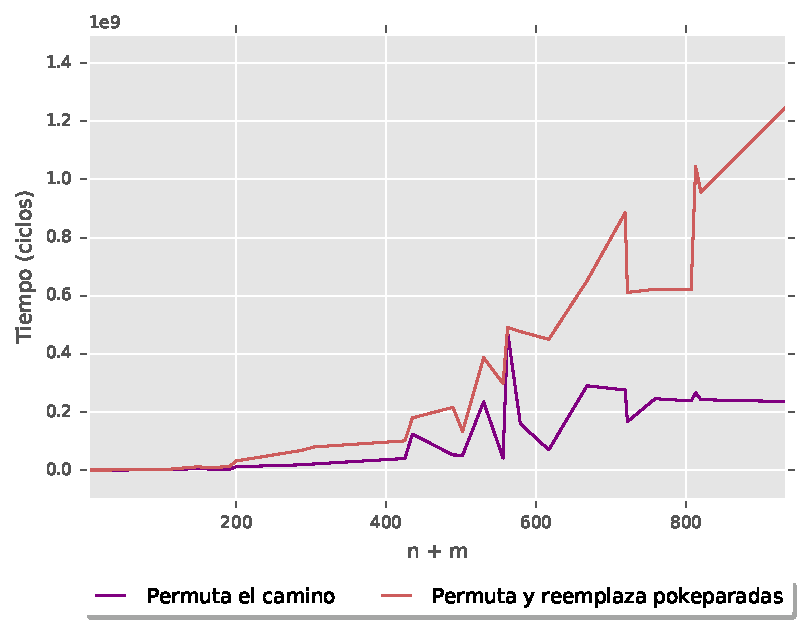
\includegraphics{../experimentacion/ej3/expAleat_cantNodos_tiempo.pdf}
    \caption{expAleat cantNodos tiempo}
    \label{fig:expAleat_cantNodos_tiempo}
  \end{center}
\end{figure}

\begin{table}[H]
    \begin{center}
        \begin{tabular}{ | l | l | l | l | l | }
            \hline
            \multicolumn{1}{|c|}{}&
            \multicolumn{2}{|c|}{\textbf{Instancias aleatorias}}&
            \multicolumn{2}{|c|}{\textbf{Instancias de mejor caso}}\\
            \cline{2-5}
                        &    \textit{Vecindad I}     &    \textit{Vecindad II}    &    \textit{Vecindad I}     &    \textit{Vecindad II}    \\ \hline
            Media       &   0.100376    &   0.127016    &   0.116154    &   0.807135    \\ \hline
            Desv\'io estandar       &   0.096465    &   0.135994    &   0.148876    &   0.937515    \\ \hline
            M\'inimo    &   0.000000    &   0.000000    &   0.000000    &   0.000000    \\ \hline
            M\'aximo    &   0.280713    &   0.484252    &   0.492888    &   2.524617    \\ \hline
        \end{tabular}
    \end{center}
    \caption{Error relativo.}    
    \label{table:error_relativo}
\end{table} 


\newpage

\section{Ejercicio IV: Metaheur\'istica}

\subsection{Introducci\'on}

Con el objetivo de mejorar las soluciones obtenidas hasta el momento con las heuristicas constructivas golosas y la de búsqueda local, decidimos implementar una metaheuristica GRASP (\textit{Greedy Randomized Adaptatative Search procedures}), esta es una metaheuristica que consiste en construir soluciones iterativamente en base a otras heuristicas quedandose con la mejor de todas las obtenidas. Cada iteración consta fundamentalmente de dos fases una parte constructiva golosa/aleatoria y otra de búsqueda local, esto se repetira hasta cumplir con un cierto críterio de parada.

\subsection{Algoritmo}

El algoritmo implementando de GRASP consta de un ciclo principal donde en cada iteración construimos una solución factible del problema con una heuristica constructiva en base a los parámetros $\alpha$ y $\omega$, estos parámetros indicaran lo golosa o aleatoria que deberá ser la solución, al resultado de la heuristica lo refinamos aplicándole búsqueda local considerando una cierta vecindad y comprobamos si el resultado mejoro con respecto a la mejor solución obtenida hasta el momento para conservarla, luego el ciclo se repite si el criterio de parada no fue alcanzado. Inicialmente recibimos como parámetros un criterio de parada del algoritmo, los valores $\alpha$ y $\omega$ y una semilla que usaremos para generar números pseudoaleatorios, en pseudocódigo tenemos lo siguiente:


\begin{algorithm}[H]

\label{}
\caption{Ciclo principal de GRASP}

\begin{algorithmic}[1]

\Statex \underline{Entrada}: Criterio de parada, $\alpha$, $\omega$, semilla
\medskip
\State mejorSoluci\'on $\gets$ $\emptyset$
\While{Criterio de parada no satisfecho}
    \State soluci\'onHeur\'istica $\gets$ ConstruirSoluci\'onHeur\'istica($\alpha$, $\omega$)
	\State soluci\'on $\gets$ AplicarB\'usquedaLocal(soluci\'onHeur\'istica)
	\If{Distancia(soluci\'on) $<$ Distancia(mejorSoluci\'on)}
		\State mejorSoluci\'on $\gets$ soluci\'on
	\EndIf
\EndWhile
\medskip
\Statex \underline{Salida}: mejorSoluci\'on

\end{algorithmic}
\end{algorithm}

La primer fase consiste en armar una solución basada en la heuristica del ejercicio 2 pero introduciendo como cambio dos parámetros que indicaran que tan golosa es la elección de elementos. Primero vamos a considerar un camino de todos los gimnasios que tendremos que recorrer, todos estos serán nuestros candidatos a incorporar a la solución y le asignaremos a cada uno de ellos un 'costo incremental' a partir de una evaluación greedy, este costo incremental representa que tanto nos cuesta agregar el elemento a la solución que estamos armando y esta determinado por la distancia del elemento con el último agregado a la lista, inicialmente sera cero si no hay elementos en la lista. Luego a partir de todos nuestros candidatos creamos una nueva lista de candidatos restringidos formada por los mejores candidatos de todos, es decir los que tienen menor costo incremental para incorporarse a la solución (parte greedy del algoritmo), de esta lista de candidatos restringidos tomamos uno al azar (parte probabilística) y lo incorporamos al camino que estamos construyendo y todos los costos incrementales del resto de los candidatos son vueltos a evaluar (parte adaptativa). En pseudocódigo:

\begin{algorithm}[H]

\label{}
\caption{Construir camino de gimnasios}

\begin{algorithmic}[1]

\Statex \underline{Entrada}: $\alpha$
\medskip
\State camino $\gets$ $\emptyset$
\State candidatos $\gets$ gimnasios
\While{Hay gimnasios restantes para agregar al camino}
    \State EvaluarCostos(candidatos)
	\State mejoresCandidatos $\gets$ CandidatosRestringidos(candidatos, $\alpha$)
	\State gimnasio $\gets$ ObtenerGimnasioAleatorio(mejoresCandidatos)
	\State Agregar(gimnasio, camino)
\EndWhile
\medskip
\Statex \underline{Salida}: camino

\end{algorithmic}
\end{algorithm}

Para la elección de los candidatos restringidos vamos a considerar sobre todos los candidatos el valor $costo_{min}$ al que tenga menor costo incremental y $costo_{max}$ al de mayor costo luego la lista restringida esta formada por los candidatos $c$ tal que $costo(c) \in [costo_{min}, costo_{min} + \alpha * (costo_{max} - costo_{min})]$, este intervalo depende del parámetro $\alpha$ donde $\alpha \in [0..1]$. La elección de un $\alpha = 0$ corresponde al intervalo $[costo_{min}, costo_{min}]$ es decir los candidatos serán elegidos de forma puramente golosa mientras que con $\alpha = 1$ el intervalo sera $[costo_{min}, costo_{max}]$ equivalente a una elección puramente aleatoria, luego el parámetro $\alpha$ regula que tan aleatoria o golosa sera la solución en cuestión.

\begin{algorithm}[H]

\label{}
\caption{Candidatos restringidos}

\begin{algorithmic}[1]

\Statex \underline{Entrada}: candidatos, $\alpha$
\medskip
\State costoM\'in $\gets$ CalcularCostoM\'in(candidatos)
\State costoM\'ax $\gets$ CalcularCostoM\'ax(candidatos)
\State candidatosRestringidos $\gets$ $\emptyset$
\For{c : candidatos}
	\If{Costo(c) $\in$ [costoM\'in, costoM\'in + $\alpha$ $\times$ (costoM\'ax - costoM\'in)]}
		\State Agregar(c, candidatosRestringidos)
	\EndIf
\EndFor
\medskip
\Statex \underline{Salida}: candidatosRestringidos

\end{algorithmic}
\end{algorithm}

Con el camino de gimnasios debemos seleccionar las pokeparadas necesarias que debemos visitar para ir recorriendo el camino de gimnasios, para ello vamos a repetir el mismo procedimiento con algunas consideraciones. Primero tomamos el primer gimnasio a recorrer de nuestro camino construido y mientras nos falten pociones para visitarlo vamos a tomar todas las pokeparadas no visitadas como candidatos y le pondremos un costo incremental de la distancia entre esa parada y el gimnasio, nuevamente obtenemos los candidatos restringidos entre todos según el parámetro $\alpha$, y de estos tomamos uno al azar, así hasta recolectar las cantidad de pociones necesarias para visitar al gimnasio y proceder con el siguiente actualizando los costos y volviendo a repetir el ciclo hasta que no queden gimnasios por recorrer. La nueva consideración a tener cuenta es el parámetro $\omega$ que cumple la siguiente función, cuando vamos visitando el camino de gimnasios tomando las pokeparadas necesarias para vencerlo queremos flexibilizar que tanto podemos desviarnos del camino recolectando algunas pociones extra si caben en la mochila, esto representa el parámetro $\omega$ con $\omega \in [0..1]$ la probabilidad de visitar otras paradas adicionalmente de las necesarias, por lo tanto cuando $\omega = 0$ en el camino se recolectaran unicamente las pociones justas para derrotar al gimnasio y pasar al siguiente, cuando $\omega = 1$ siempre se desviara hasta llenar la mochila. Finalmente la construcción de la solución heuristica es:

\begin{algorithm}[H]

\label{}
\caption{Construir soluci\'on heur\'istica}

\begin{algorithmic}[1]

\Statex \underline{Entrada}: $\alpha$, $\omega$
\medskip
\State caminoGimnasios $\gets$ ConstruirCaminoGimnasios($\alpha$)
\State soluci\'on $\gets$ $\emptyset$
\State pociones $\gets$ $0$
\State candidatos $\gets$ pokeparadas

\While{Hay gimnasios en caminoGimnasios}
	\While{pociones $<$ Poder(Pr\'ox(caminoGimnasios)) $\lor$ (pociones $<$ mochila $\land$ BoolRnd($\omega$))}
		\State EvaluarCostos(candidatos)
		\State MejoresCandidatos $\gets$ CandidatosRestringidos(candidatos, $\alpha$)
		\State pokeparada $\gets$ ObtenerPokeparadaAleatoria(mejoresCandidatos)
		\State Agregar(pokeparada, soluci\'on)
		\State pociones $\gets$ M\'inimo(pociones$+3$, mochila)
	\EndWhile
	\State pociones $\gets$  pociones $-$ Poder(Pr\'ox(caminoGimnasios))
	\State  Agregar(Pr\'ox(caminoGimnasios), soluci\'on)
	\State  SacarPrimero(caminoGimnasios)
\EndWhile

\medskip
\Statex \underline{Salida}: soluci\'on

\end{algorithmic}
\end{algorithm}

En la segunda fase a esta solución le aplicamos la heuristica de búsqueda local implementada eligiendo alguna vecindad. Luego introducimos dos criterios de paradas en el algoritmo:

\paragraph{Criterio I: Iteraciones fijas}
Dado un parámetro $K$ este criterio consiste en interpretar a $K$ como la cantidad de exactas de iteraciones que tendrá el ciclo principal hasta concluir el algoritmo y devolver la solución obtenida.

\paragraph{Criterio II: Iteraciones sin mejoras}
En este criterio de parada es consideramos a $K$ como las iteraciones máximas efectuadas del ciclo sin lograr mejorar la solución obtenida.


\subsubsection{Complejidad}

Consideramos como parámetros de entrada $G$ cantidad de gimnasios, $P$ cantidad de paradas y $K$ cantidad de iteraciones con el criterio de parada de iteraciones fijas.
El algoritmo consta de un ciclo principal que realiza exactamente $K$ iteraciones en cada iteración llama a una función que construye la solución heuristica y luego le aplica búsqueda local esto es \bigo{K * costo(Heuristica) * costo(Busqueda Local)} 

Para construir nuestra solución heuristica lo primero que realizamos es la construcción de un camino de gimnasios utilizando la función graspSolucionGimnasios, en esta función iteramos sobre la cantidad total de gimnasios y en cada iteración actualizamos todos los gimnasios que son candidatos recorriendolos todos nuevamente y haciendo operaciones de costo constante como actualizar su costo incremental, luego a estos candidatos los procesamos con la función obtenerCandidatosRestringidos pero esta función tiene costo lineal sobre los candidatos recibidos, por lo tanto todo el costo es de \bigo{G*(G+G)} $\in$ \bigo{G^2}.

La segunda parte de la heuristica se hace llamando a graspSolucionAleatoria en base a un camino de gimnasios de longitud $G$, itera sobre todos los gimnasios del camino y en cada iteración obtiene las paradas que son necesarias visitar el gimnasio actual, la cantidad de paradas que se visitaran entre todos los gimnasios serán como máximo $P$, y en cada parada visitada se actualiza el costo incremental de todas, esto es \bigo{G+P*P}. Finalmente el costo total de la heuristica es de \bigo{G^2+G+P^2} $\in$ \bigo{G^2+P^2}.

Por lo tanto La complejidad temporal de todo el algoritmo es del orden \bigo{K*(G^2+P^2)*costo(Busqueda Local)}




\newpage

\section{Ejercicio V: Comparaci\'on de algoritmos}

Realizamos mediciones sobre instancias aleatorias generadas como describimos en la secci\'on \ref{sec:ej3_exp_instancias}, en particular, instancias chicas para poder ejecutar el algoritmo de backtracking.

Con los datos obtenidos graficamos las distancias obtenidas con cada algoritmo, en cada instancia estudiada, en la figura \ref{fig:ej5_expAleatOp_instancia_distancia}.

\begin{figure}[H]
  \begin{center}
    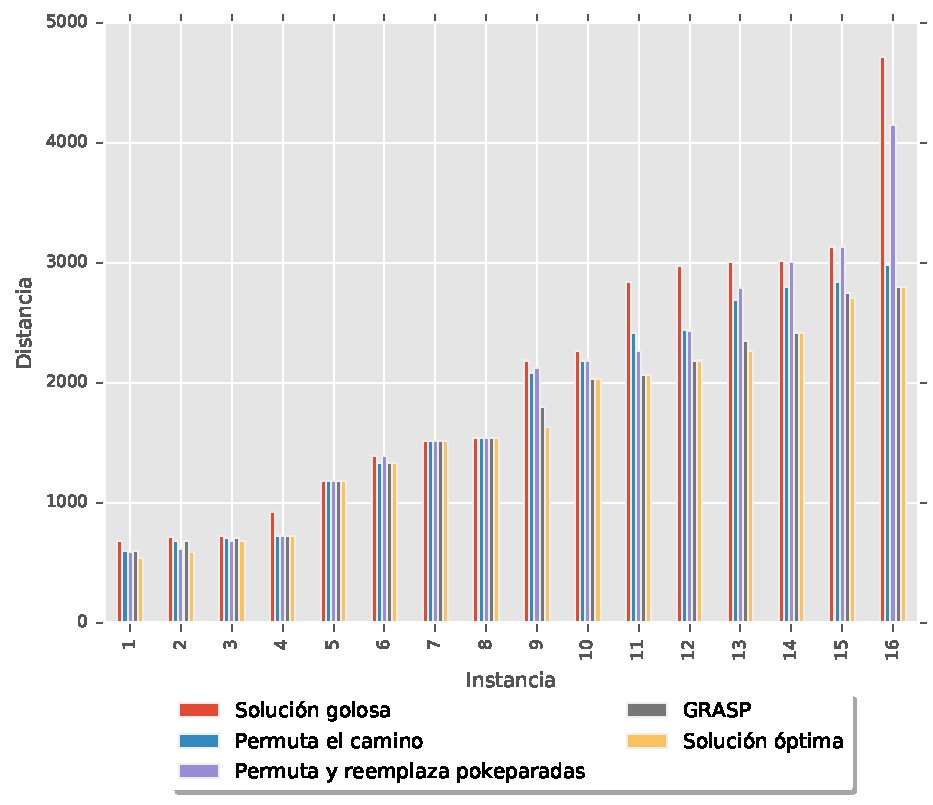
\includegraphics{../experimentacion/ej5/expAleatOp_instancia_distancia.pdf}
    \caption{Distancias computadas para cada una de las instancias analizadas, utilizando instancias aleatorias.}
    \label{fig:ej5_expAleatOp_instancia_distancia}
  \end{center}
\end{figure}

\begin{figure}[H]
  \begin{center}
    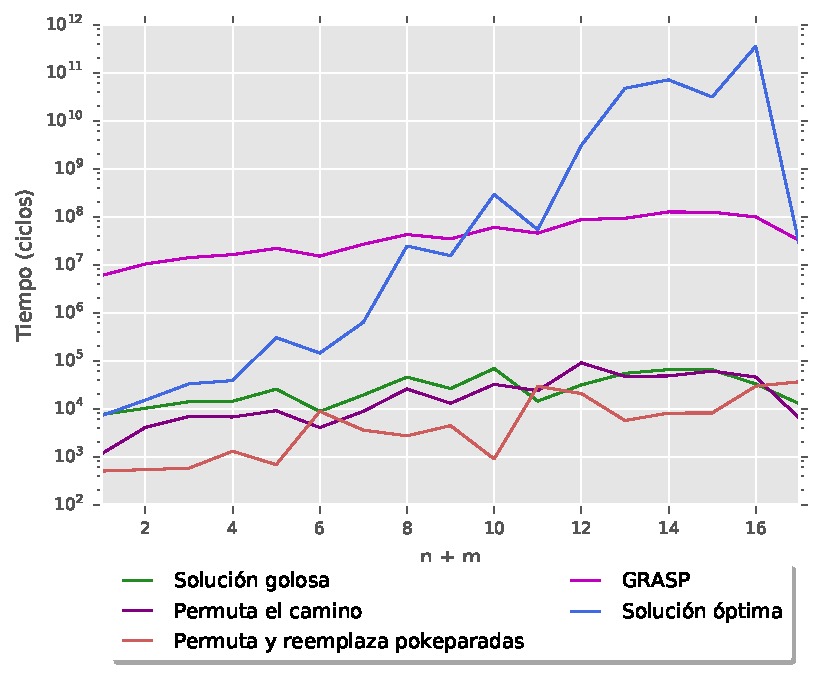
\includegraphics{../experimentacion/ej5/expAleatOp_cantNodos_tiempo.pdf}
    \caption{Tiempo en funci\'on de la cantidad de nodos usando instancias aleatorias.}
    \label{fig:ej5_expAleatOp_cantNodos_tiempo}
  \end{center}
\end{figure}

Exihibimos a continuaci\'on un conjunto de nodos ejemplo del problema, junto con los caminos determinados por los algoritmos desarollados a lo largo de este trabajo:

\begin{figure}[H]
\centering
\begin{minipage}{0.45\textwidth}
\centering
    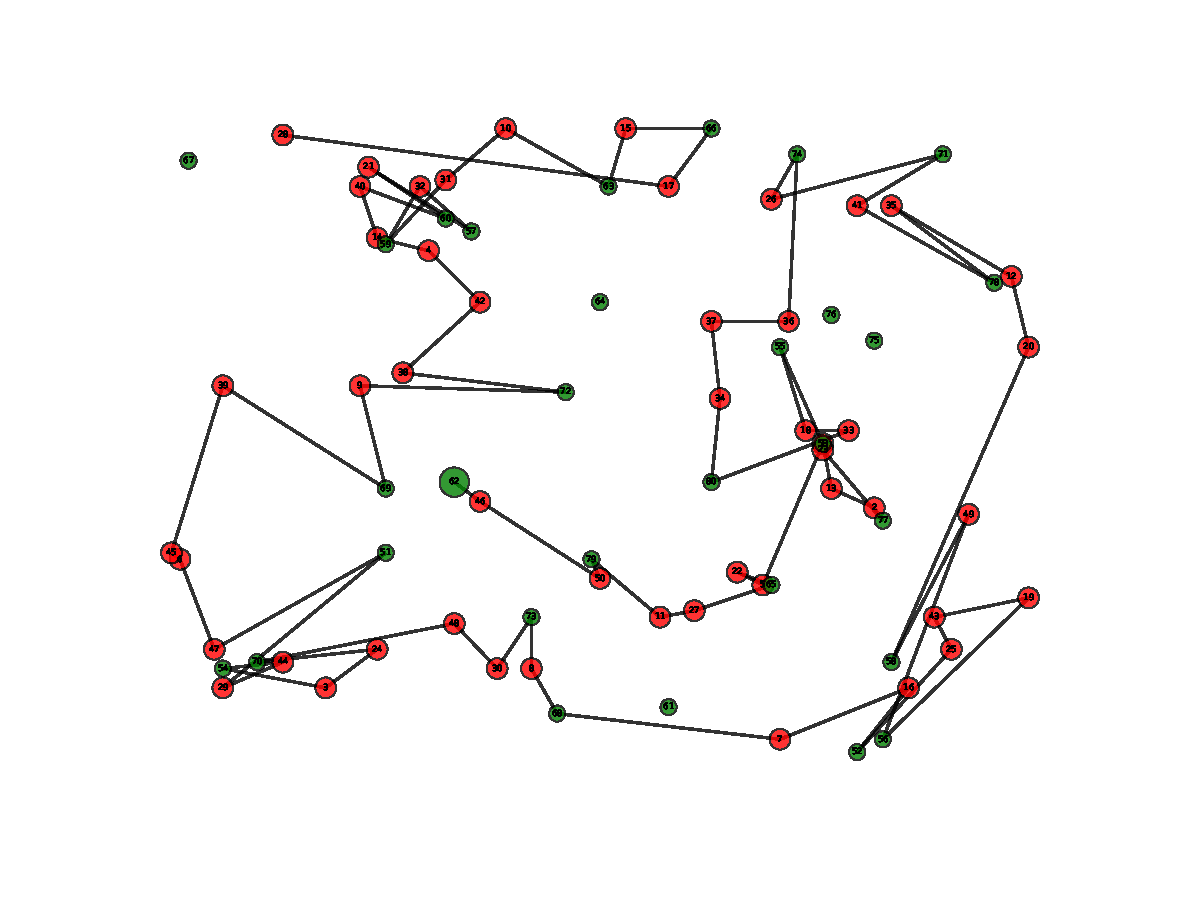
\includegraphics[scale=0.4]{../experimentacion/ej5/ejemplo-salidaSG.pdf}
    \caption{Algoritmo goloso}
    \label{fig:ejemplo-salidaSG}
\end{minipage}
\qquad
\begin{minipage}{0.45\textwidth}
\centering
    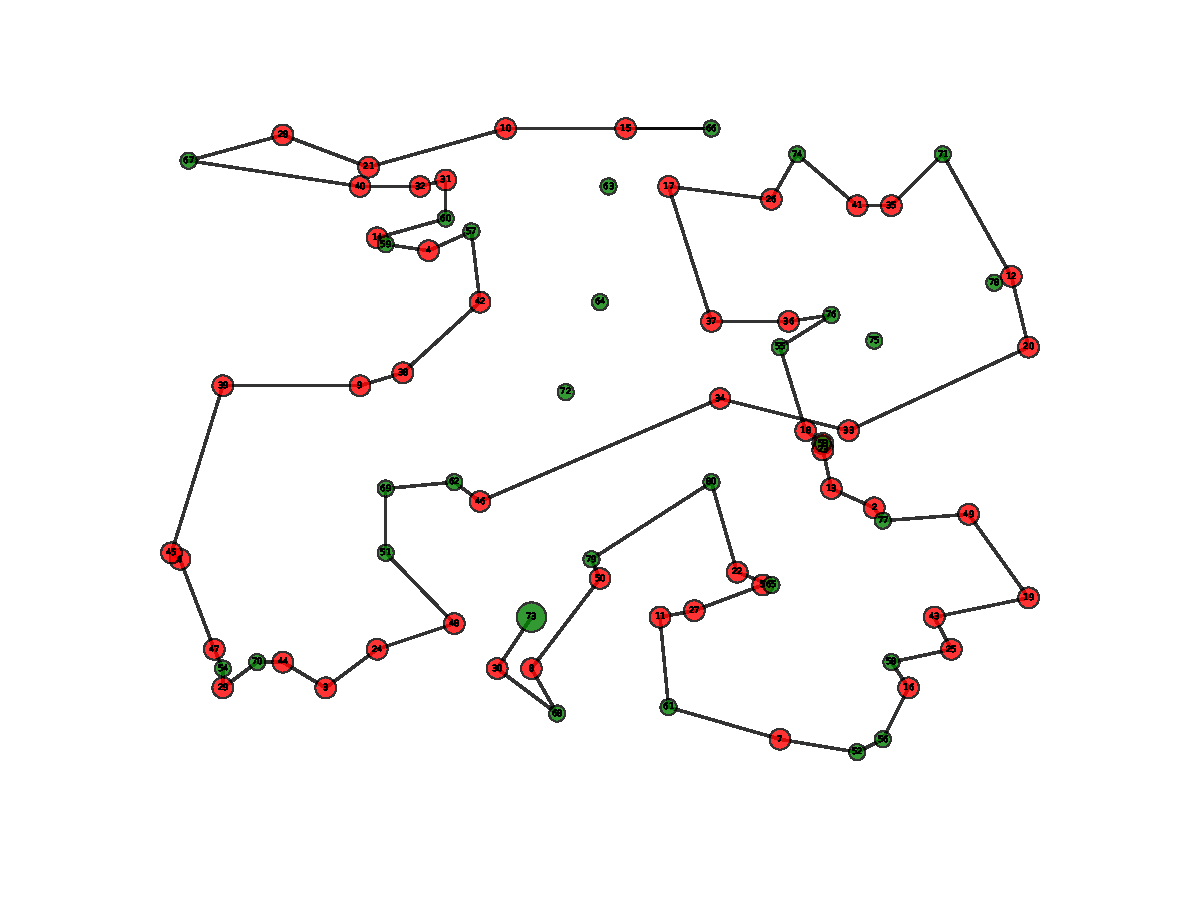
\includegraphics[scale=0.4]{../experimentacion/ej5/ejemplo-salidaGRASP.pdf}
    \caption{GRASP}
    \label{fig:ejemplo-salidaGRASP}
\end{minipage}
\end{figure}

\begin{figure}[H]
\centering
\begin{minipage}{0.45\textwidth}
\centering
    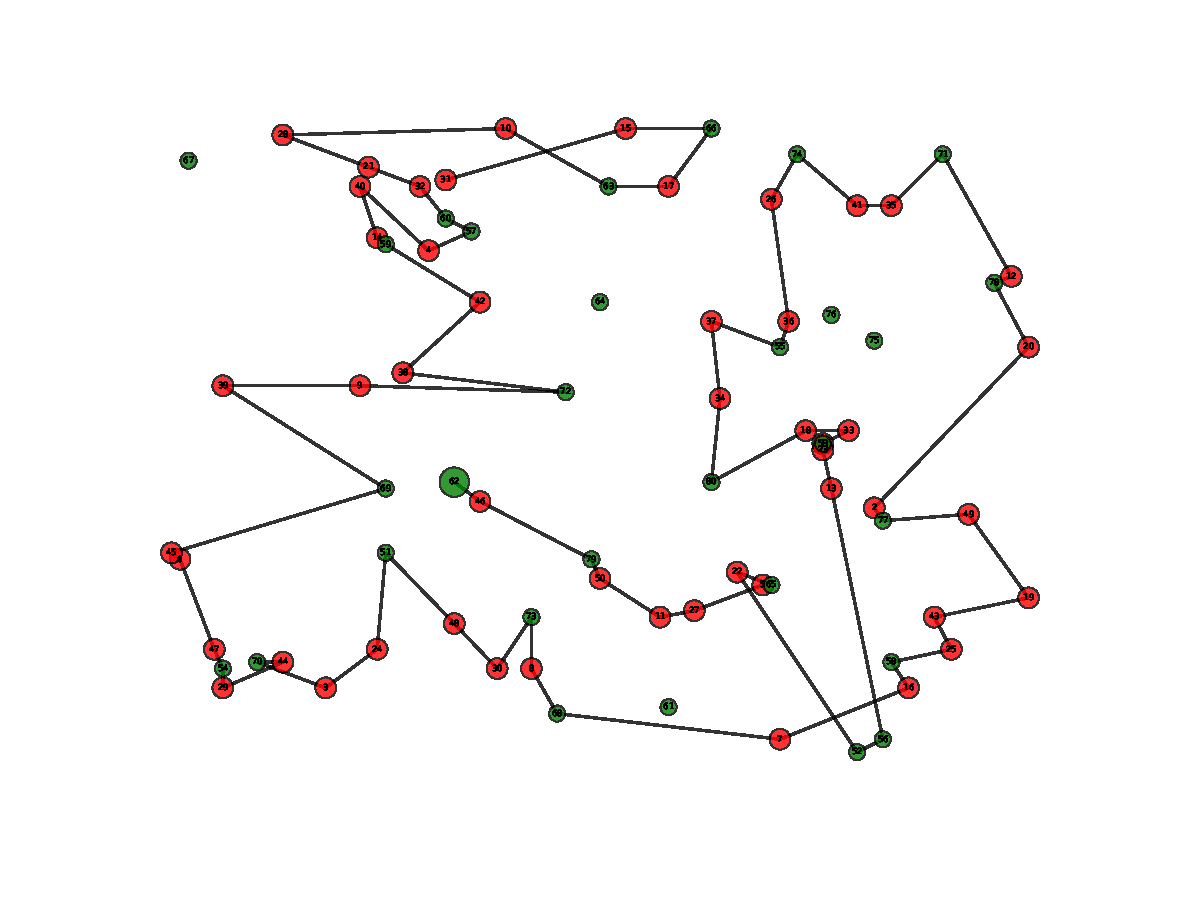
\includegraphics[scale=0.4]{../experimentacion/ej5/ejemplo-salidaBLPC.pdf}
    \caption{B\'usqueda local permutando el camino}
    \label{fig:ejemplo-salidaBLPC}
\end{minipage}
\qquad
\begin{minipage}{0.45\textwidth}
\centering
    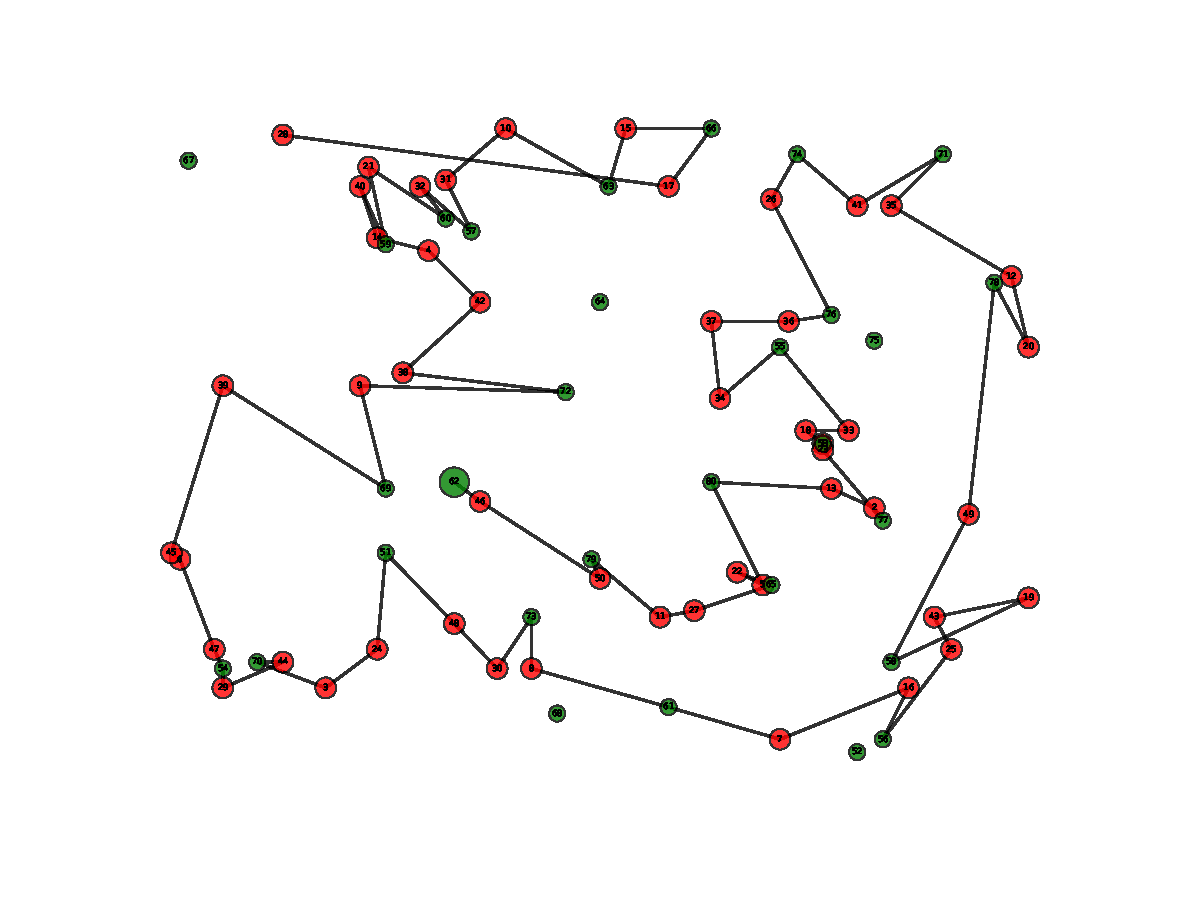
\includegraphics[scale=0.4]{../experimentacion/ej5/ejemplo-salidaBLPYRP.pdf}
    \caption{B\'usqueda local permutando y reemplazando pokeparadas}
    \label{fig:ejemplo-salidaBLPYRP}
\end{minipage}
\end{figure}

\end{document}